\documentclass[11pt,a4paper]{article}
\usepackage[margin=2.3cm]{geometry}
\usepackage[T1]{fontenc}
\IfFileExists{lmodern.sty}{\usepackage{lmodern}\usepackage{microtype}}{\usepackage[expansion=false]{microtype}}
\usepackage{amsmath,amssymb,amsthm}
\usepackage{booktabs,tabularx,array,longtable,multirow}
\usepackage{enumitem}
\usepackage{xcolor}
\usepackage{tikz}
\usetikzlibrary{positioning,arrows.meta,fit,calc,shapes.misc}
\usepackage{pgfplots}\pgfplotsset{compat=1.16}
\usepackage[hidelinks]{hyperref}
\setlist{itemsep=2pt,topsep=4pt}
\setlength{\emergencystretch}{3em}
\newcolumntype{L}{>{\raggedright\arraybackslash}X}
\newcommand{\flag}[1]{\texttt{#1}}
\newtheorem{proposition}{Proposition}
\newcommand{\rotl}[1]{\mathrm{ROTL}^{#1}}
\tikzset{
  nd/.style={draw,rounded corners=2pt,align=center,font=\footnotesize,inner sep=4pt,minimum height=0.9cm},
  src/.style={nd,fill=blue!8},
  ref/.style={nd,fill=orange!12},
  term/.style={nd,fill=green!10},
  joinnd/.style={nd,fill=green!10,double},
  ed/.style={-{Stealth[length=2.2mm]},thick},
  el/.style={font=\scriptsize,fill=white,inner sep=1pt}
}

\begin{document}
\begin{titlepage}
\centering
\vspace*{3cm}
{\Huge\bfseries Compositional SAT Search with Dagster\par}
\vspace{0.6cm}
{\Large Preimages of 22-Round SHA-1: a Scheduler Patch\\and a Locked Confirmatory Evaluation\par}
\vspace{1.5cm}
{\Large Virtual Proceedings of an Investigation\par}
\vspace{2cm}
{\large Charles Gretton\textsuperscript{$\ast$}\par}
{\normalsize Australian National University\par}
\vspace{1cm}
{\normalsize November 2026\par}
{\small Release 1.0\par}
\vfill
{\small\textsuperscript{$\ast$}Corresponding author:
\href{mailto:charles.gretton@anu.edu.au}{charles.gretton@anu.edu.au}\par}
\end{titlepage}

\begin{abstract}
This report studies how to organise a many-core Boolean satisfiability (SAT) search for preimages
of 22-round SHA-1, and is written from first principles: it defines the operators, the reduced-round
compression function, its translation to conjunctive normal form, conflict-driven SAT solving and
Dagster's message-passing execution model before presenting the experiment.

The method is a sound coarse-to-fine search expressed as a Dagster graph. A source node solves a
\emph{relaxation}, the subset of the exact formula's clauses that computes only the low-order $k$
bits of each modular addition. Every exact SHA-1 execution satisfies it, because it is a subset.
Carry direction makes the retained low-bit slice self-contained, with a known carry-in of zero. In
the measured instances the resulting trans-round traces also filtered strongly, with only a small
fraction extending to a full preimage. A terminal node holding the exact formula tries to extend
each trace; in the most effective pipeline an intermediate node first refines 8-bit traces to
16 bits. Every reported preimage is checked by an independent forward implementation of SHA-1.

At 22 rounds the three-stage pipeline exposed a scheduler failure, the \emph{refinement lock}:
intermediate refinements never complete, fill Dagster's finite work buffer, and starve the exact
checks. An opt-in retirement threshold $L$ removes it. Role-specific conflict budgets were also
tested and found to reduce performance, so they were disabled.

With $L=8$ frozen after development-only tuning, on three untouched targets the compositional race
found a verified preimage in all 30 runs (median 26.9\,s on 64 worker cores), against 28 of 30 for
observed 64-process portfolios of the same MiniSat~2.2 solver (median 552.6\,s). It was faster in
all 30 paired runs (sign test $p=1.9\times10^{-9}$). The result is relative to a MiniSat portfolio:
one single-core CryptoMiniSat run solved a 22-round target in 397\,s, so a portfolio of a stronger
solver is a materially stronger, still untested, baseline. No claim is made about full 80-round
SHA-1 or its security.
\end{abstract}

\tableofcontents
\newpage

\section*{Licence and errata}
\addcontentsline{toc}{section}{Licence and errata}

\paragraph{Licence.} Copyright 2026 Charles Gretton. This work is licensed under the Creative Commons
Attribution 4.0 International licence (CC BY 4.0). To view a copy of the licence, visit
\url{https://creativecommons.org/licenses/by/4.0/}. The software released with it in the sha1-dagster
repository is licensed under the Apache License, Version 2.0
(\url{https://www.apache.org/licenses/LICENSE-2.0}), except two components derived from third-party
software under the GNU General Public License: the instance generator, a modified copy of
\texttt{sha1-sat} \cite{nossum} (GPL-3.0-or-later, Copyright Vegard Nossum), and a seeded TiniSAT
engine derived from Dagster (GPL-2.0-or-later). Material by others that is cited or used here,
including Dagster, MiniSat and the Dagster source quoted in Appendix~\ref{app:patch}, remains under
its original terms.

\paragraph{Errata.} We welcome reports of errors, omissions and overlooked prior work. Please send them to the
corresponding author, Charles Gretton, at \href{mailto:charles.gretton@anu.edu.au}{charles.gretton@anu.edu.au}.
Every report that leads to a correction will be acknowledged in the errata and in any revised edition,
cited as a private communication; where the point was already made in a publication that appeared before
this report's publication date, that publication will be cited as well.

\section*{AI usage acknowledgment}
\addcontentsline{toc}{section}{AI usage acknowledgment}

Large language models, including Claude Opus 5.5, were used extensively throughout this investigation
and in preparing this volume. Their use covered developing and checking arguments; designing,
writing, testing and running the software; planning, monitoring and analysing the computational
campaigns; and drafting, reviewing and revising the text, including assembling these proceedings from
the project's reports.

The author directed the work, decided what to run and what to claim, and checked its major claims.
He has not made a complete inventory of the claims in this volume, nor checked each one individually,
so errors may remain, and reports of them are welcome (see the errata above). What the volume provides
instead is the means to check: each computational claim rests on released software and recorded
outputs, and the report states how its claims were checked. The use of models also shaped the
methods. Much of the emphasis on independent verification of every preimage, fail-closed launch and
patch checks, the separation of development from evaluation targets, the coded list of what remains to be
established (Section~\ref{sec:future}) and the explicit withdrawal of a claim found to be wrong
(Section~\ref{sec:protocol}) exists so
that results produced with heavy machine assistance can be audited without trusting the process that
produced them.

The author calls a release of this kind a \emph{virtual proceedings}: a self-contained manuscript
published together with the code package that produced its results --- the volume and its source,
the software needed to rerun every experiment, and the derived evidence behind every reported
number --- as one open repository rather than through a conventional venue. The name reflects both
how such work is now produced, largely in dialogue with AI tools under the author's direction, and
how it is meant to be used: read, rerun and audited by others.

\section*{Preface}
\addcontentsline{toc}{section}{Preface}

This volume reports one investigation: whether a sound, structure-following decomposition of a hard
SAT problem, run by the Dagster distributed solver, finds solutions faster than a conventional
portfolio of the same solver, and what had to change in Dagster for it to do so. The problem is
finding preimages of SHA-1 reduced to 22 rounds. The volume is self-contained: every notion is
introduced from first principles, and every number in the results is backed by derived tables,
validation outputs and checksums released with it. The sha1-dagster repository holds the volume's
source, the instance generator, the Dagster patch, the experiment harness, the analysis software and
that evidence. Dagster itself, MiniSat and their dependencies are obtained from their own
repositories. Every experiment ran on a single 64-core workstation, apart from one supplementary
single-solver measurement on a separate one-core machine.

\newpage

%=============================================================================================
\section{Introduction}\label{sec:intro}
%=============================================================================================

\subsection{Satisfiability solving}

A Boolean variable takes the value true or false. A \emph{clause} is an ``or'' of variables or their
negations, such as $(x_1 \vee \neg x_2 \vee x_3)$, which is satisfied when at least one of its parts
is true. A formula in \emph{conjunctive normal form} (CNF) is an ``and'' of clauses. The
satisfiability problem asks whether some assignment satisfies every clause at once, and if so, which
one. The problem is NP-complete, so no method is known that is fast on every formula. Yet modern
solvers routinely handle formulas with millions of clauses arising in hardware verification,
planning and scheduling, by searching cleverly and learning from their own dead ends
(Section~\ref{sec:background}).

Almost any finite computation can be written as such a formula. Each bit computed becomes a variable,
and each step becomes clauses forcing the output bits to agree with the input bits. Fixing the
desired \emph{output} bits and asking a solver for the \emph{input} bits runs the computation
backwards.

\subsection{Hash functions as a benchmark}

A cryptographic hash function such as SHA-1 maps any message to a short fixed-length fingerprint,
160 bits for SHA-1. It is designed to be easy to compute forwards and infeasible to invert: given a
fingerprint, it should be impractical to find any message (a \emph{preimage}) producing it. SHA-1
reaches this by applying a round of mixing operations 80 times. Restricting it to its first $r$ rounds
gives a family of problems whose difficulty grows steeply with $r$. These problems make a good
benchmark for three reasons:
\begin{itemize}
\item \textbf{They are hard but tunable.} Adding one round makes the problem much harder, so a method's
reach can be measured by the number of rounds at which it still succeeds.
\item \textbf{Answers are instantly checkable.} A claimed preimage is verified by computing the hash
forwards, so a correct answer cannot be faked.
\item \textbf{They are standard and reproducible.} Instances are generated from a seed by a public tool.
\end{itemize}
Nothing in this report threatens SHA-1. The full 80-round function is untouched, and published
cryptanalysis reaches far more rounds than are studied here. The point is to measure \emph{how to
organise a parallel search}, using a problem whose difficulty is well understood.

\subsection{Using many cores}

A modern machine has dozens of cores. The simplest way to use them on one SAT problem is a
\emph{portfolio}: run independent copies of the same solver with different random seeds and stop
when the first finishes. Run times on hard problems vary enormously between seeds, so the fastest of
64 copies can be far faster than a typical one. The portfolio is simple and robust, but the copies
learn nothing from each other's work.

The alternative is to \emph{decompose} the problem and have different cores work on different
parts. The obvious way, fixing some variables to each of their possible values and giving each
combination to a core (``cube and conquer''), often fails on cryptographic problems: forcing a few
bits of a hash computation can make each piece harder than the whole. A useful decomposition has to
follow the problem's structure.

\subsection{Dagster and the idea studied here}

Dagster \cite{burgess2022dagster,burgess2023dagster} lets a user describe a decomposition as a \emph{directed acyclic graph}. Each
node holds a subset of the formula's clauses. When a node is solved, the values of the variables it
shares with the next node are passed along an edge as a message, and the next node solves its own
clauses with those values fixed. A scheduler assigns the resulting pieces of work to cores.

The decomposition studied here exploits the arithmetic inside SHA-1. Each round adds 32-bit numbers,
and in binary addition the low-order bits of a sum depend only on the low-order bits of the inputs,
since carries flow upwards, never downwards. Keeping only the clauses for the lowest 16 bits of every
addition gives a smaller, easier formula, a \emph{relaxation}. Every true preimage satisfies it,
since it is part of the full formula. Because carries flow upwards, the low-bit slice is also
self-contained: it starts from a known carry of zero and needs nothing from the discarded high bits,
which is what makes it an effective filter. Its solutions are cheap \emph{candidates}, here called \emph{traces}. A second node
holding the complete formula checks each candidate, either extending it to a full preimage or
rejecting it, usually within milliseconds. This is like checking that the last few digits of a long
sum come out right before checking the rest: most wrong answers are discarded cheaply. How strongly
this filters is an empirical property of these instances, not a consequence of the arithmetic
alone. In the 21-round measurements only about 0.3--0.4\% of relaxation traces extended to a
preimage, and the median rejection took about 0.4\,ms.

Dagster can race several such pipelines at once. The one that proved most effective has three
stages: an 8-bit relaxation proposes coarse candidates, a 16-bit stage refines them, and the exact
formula checks the result.

\subsection{What went wrong, and what this report does}

At 21 rounds every method finished within seconds, too quickly to tell them apart. At 22 rounds the
three-stage pipeline usually stalled. Its middle stage never declares that it has finished refining
a candidate, because there are always more refinements to try. Dagster's scheduler keeps a fixed
number of jobs in its queue, so the unfinished middle-stage jobs eventually occupy every place, and
no candidate ever reaches the final check. The cores keep producing refinements that nothing
examines. We call this the \emph{refinement lock}.

This report:
\begin{enumerate}
\item explains SHA-1, its encoding as SAT, and the history of approaches that led to the
staged pipeline (Section~\ref{sec:background});
\item sets out every pipeline design explored, with schematics of what each stage contains
(Section~\ref{sec:dags});
\item describes in detail a small, optional change to Dagster that lets a middle stage retire a
candidate after a set number of refinements, which removes the lock (Section~\ref{sec:method});
\item evaluates the change in three phases: a check that the patched solver behaves like the original
when the change is switched off; tuning on two problems; and a final evaluation, with every setting
fixed in advance, on three problems never used for tuning, against a portfolio of the same solver
running on the same 64 cores (Sections~\ref{sec:protocol}--\ref{sec:phaseC});
\item states precisely what is and is not established, as a coded list of open questions
(Section~\ref{sec:future}).
\end{enumerate}


\paragraph{How to read this report.}
Section~\ref{sec:background} defines all operators, notation, SHA-1 equations, SAT concepts and
Dagster semantics used later. The summary of results follows that background, so the headline
numbers can be interpreted without relying on unstated implementation knowledge. Subsequent
sections describe every DAG family, the retirement patch, the locked experimental protocol,
development-only tuning, untouched-target evaluation, limitations and exact reproduction steps.

Every answer reported was checked by recomputing SHA-1, independently of the solver that found it.

%=============================================================================================
\section{Background}\label{sec:background}

\subsection{Conventions, operators and notation}\label{sec:notation}

\paragraph{Bits, words and indexing.}
A \emph{bit} is an element of $\mathbb B=\{0,1\}$. A 32-bit word is an element of
$\mathbb B^{32}$ and is also interpreted as an unsigned integer in
$\mathbb Z_{2^{32}}=\{0,\ldots,2^{32}-1\}$. For a word $X$, $X[i]$ denotes bit $i$, with
$X[0]$ the least significant bit and $X[31]$ the most significant bit. A slice
$X[i..j]$ contains bits $i,i+1,\ldots,j$. Hexadecimal constants are written with the most
significant digit first, following the SHA-1 standard.

\paragraph{Three meanings of ``message''.} To avoid ambiguity, the \emph{message block} is SHA-1's
512-bit input; a \emph{Dagster message} (or \emph{trace message}) is a projected partial assignment
passed along a DAG edge; and an \emph{MPI record} is a transport-level communication between
processes. The \emph{message schedule} keeps its standard name.

\paragraph{Boolean operators.}
For bits $x,y\in\mathbb B$:
\begin{align*}
\neg x &\text{ is logical negation}, &
 x\wedge y &\text{ is conjunction},\\
 x\vee y &\text{ is disjunction}, &
 x\oplus y &\text{ is exclusive-or}.
\end{align*}
The operators act bitwise when applied to words. Exclusive-or is addition modulo two on each bit:
$x\oplus y=1$ exactly when $x\ne y$. We use $\bigwedge$ and $\bigvee$ for conjunction and
disjunction over indexed families.

\paragraph{Word operations.}
For 32-bit words $X$ and $Y$:
\begin{itemize}
\item $X\boxplus Y$ is unsigned addition modulo $2^{32}$; overflow beyond bit 31 is discarded;
\item $X\oplus Y$, $X\wedge Y$, $X\vee Y$ and $\neg X$ are bitwise operations;
\item $\rotl{n}(X)$ rotates $X$ left by $n$ positions:
\[
  \rotl{n}(X)[i]=X[(i-n)\bmod 32].
\]
A rotation changes wiring but introduces no new arithmetic constraint in a bit-level encoding.
\end{itemize}
The direction of carry propagation is important. In ordinary binary addition, output bit $i$ depends
only on input bits $0..i$ and carries generated below $i$; higher input bits cannot affect a lower
output bit. Retaining only the constraints at positions $0..k-1$ therefore gives a low-$k$
slice of an adder that is \emph{exact} for those positions: with carry-in zero at bit 0, it determines
output bits $0..k-1$ from input bits $0..k-1$ alone. (Any subset of an exact formula's clauses is
sound, in that every exact model satisfies it. The carry direction is what makes the low slice
self-contained. An interior slice $i..i+k-1$ with $i>0$ has an unknown carry-in, which is why such
slices were measured to make the search harder rather than easier.) Note that rotations move
high-order bits of earlier words into low positions: $\rotl{5}(A)[0..4]=A[27..31]$. A low-$k$ slice
of a round's adders therefore constrains some high bits of earlier state words through the rotated
operands.

\paragraph{SHA-1 Boolean functions.}
For 32-bit words $B,C,D$, SHA-1 uses
\begin{align*}
\mathrm{Ch}(B,C,D) &= (B\wedge C)\oplus(\neg B\wedge D),\\
\mathrm{Parity}(B,C,D) &= B\oplus C\oplus D,\\
\mathrm{Maj}(B,C,D) &= (B\wedge C)\oplus(B\wedge D)\oplus(C\wedge D).
\end{align*}
For each bit position, $\mathrm{Ch}$ chooses the corresponding bit of $C$ when $B=1$ and of $D$
when $B=0$; $\mathrm{Maj}$ returns the majority value of the three bits. In a 22-round instance,
rounds 0--19 use $\mathrm{Ch}$ and rounds 20--21 use $\mathrm{Parity}$; $\mathrm{Maj}$ (rounds
40--59) does not occur.

\paragraph{Boolean formulae and CNF.}
A Boolean variable $x$ takes a value in $\mathbb B$. A \emph{literal} is $x$ or $\neg x$. A clause
$C=(\ell_1\vee\cdots\vee\ell_m)$ is satisfied when at least one literal is true. A CNF formula
$F=C_1\wedge\cdots\wedge C_n$ is satisfied when every clause is satisfied. We write
$\mathsf{Vars}(F)$ for its variables and $\alpha\models F$ when assignment $\alpha$ satisfies $F$.
A formula is \emph{SAT} if such an assignment exists and \emph{UNSAT} otherwise.

A Tseitin encoding introduces auxiliary variables for gate outputs and adds clauses enforcing each
gate relation. For example, $z\leftrightarrow(x\wedge y)$ is encoded by
\[
  (\neg x\vee\neg y\vee z)\wedge(x\vee\neg z)\wedge(y\vee\neg z).
\]
The encoding is equisatisfiable with the circuit: every circuit execution extends to a satisfying
assignment, and every satisfying assignment agrees with the encoded gates.

\paragraph{SAT-solving terminology.}
A \emph{decision} is a solver-chosen literal. \emph{Unit propagation} assigns the remaining literal
of a clause when all its other literals are false. A \emph{conflict} occurs when every literal in a
clause is false. A conflict-driven clause-learning (CDCL) solver analyses the implication graph,
learns a clause that excludes the conflicting partial assignment, and backtracks. A \emph{model} is
a satisfying assignment. A \emph{seed} changes solver randomisation but not the formula. For MiniSat, the seed has effect
only together with random initialisation (\flag{-rnd-init}), which the portfolio arm uses.

An \emph{assumption cube} is a conjunction of literals supplied for one incremental solve. For a
variable set $Z$ and projected assignment $\pi_Z(\alpha)$, define
\[
 A(Z,\alpha)=\bigwedge_{x\in Z}\begin{cases}
 x,&\alpha(x)=1,\\
 \neg x,&\alpha(x)=0.
 \end{cases}
\]
An incremental solver preserves its original and learned clauses between calls while changing the
assumption cube.

\paragraph{Dag and Dagster notation.}
A directed acyclic graph is $G=(V,E)$, with nodes $V$ and directed edges $E\subseteq V\times V$.
Every Dagster node $v$ owns a clause subset $F_v$. An edge $e=(u,v)$ is labelled by a projection set
$Z_e$. A worker solving $u$ receives an assumption cube $A_u$ built from $u$'s incoming message
(empty for a source). When it finds a model $\alpha\models F_u\land A_u$, Dagster emits the message
$\pi_{Z_e}(\alpha)$ along each outgoing edge $e$. Node $v$ solves $F_v$ under compatible incoming
messages. A node with no parents is a \emph{source}; a node with both incoming and outgoing edges is
an \emph{intermediate}; a node with no outgoing edges is a \emph{terminal}. A node with neither, such
as the one-node \emph{direct} DAG, is both a source and a terminal. Internally, Dagster represents a
source by a self-loop reverse connection, a detail the patch relies on
(Section~\ref{sec:method}). Several incoming edges to one node form a \emph{join},
which may induce a Cartesian product of compatible parent messages.

\paragraph{Exact and relaxed SHA-1 formulae.}
$F$ denotes the complete CNF for one reduced-round preimage instance, including the fixed digest.
$R_k\subset F$ denotes the low-$k$ relaxation defined precisely in
Section~\ref{sec:dags}: it retains all constants, message-expansion and target clauses, but only the
constraints at the low $k$ bit positions of each round (its Boolean function and adders) and of the
final feed-forward additions. Every exact model satisfies every
$R_k$, but a model of $R_k$ need not extend to a model of $F$. Note that $R_k$ keeps all 160 digest
units but only the low $k$ positions of the final feed-forward adders. The digest bits at positions
$k$ and above therefore stay fixed by their unit clauses but are disconnected from the rest of
$R_k$ (or only weakly connected through rotations), so they constrain nothing there. This makes
$R_k$ looser at high bits; it does not affect soundness. The projected trans-round state bits
are denoted $z_k$: bits $0..k-1$ of each \emph{free} state word $a_5,\dots,a_{r-1}$, which is
$(r-5)k$ bits (272 bits for $k=16$ at $r=22$). Words $a_0,\dots,a_4$ are fixed by the IV, and
$a_r,\dots,a_{r+4}$ are fixed by the target digest through the feed-forward, so only
$a_5,\dots,a_{r-1}$ are unknown. A trace is therefore not a complete SHA-1 state or message; it is a partial
assignment used to condition a later exact search.

\paragraph{Targets, runs and phases.}
A target identifier such as \texttt{g10004} names one fixed 160-bit digest and its generated CNF.
The generator draws a random \emph{planted} message from the seed (here 10004) and computes its
digest, so every target is known to be satisfiable. The planted message is used only to validate DAG
constructions; it is never given to a solver.
Repeated runs on a target preserve the logical instance while changing solver seeds or runtime
interleavings. Targets \texttt{g10004} and \texttt{g10005} were used for development and parameter
selection. Targets \texttt{g10001}--\texttt{g10003} were withheld until the configuration was frozen
and were then used for the locked confirmatory evaluation.

%=============================================================================================

\subsection{SHA-1}

SHA-1 \cite{fips180} maps a message to a 160-bit digest by the Merkle--Damg{\aa}rd construction.
The message is padded and split into 512-bit blocks. A compression function updates a 160-bit
chaining state $H=(H_0,\dots,H_4)$, five 32-bit words, initialised to a fixed vector (IV). For one
block the function proceeds in three steps.

\paragraph{Message schedule.} The block supplies sixteen 32-bit words $W_0,\dots,W_{15}$. Later
words are defined linearly over $\mathrm{GF}(2)$:
\begin{equation}
W_t=\rotl{1}\!\left(W_{t-3}\oplus W_{t-8}\oplus W_{t-14}\oplus W_{t-16}\right),\qquad 16\le t<80.
\end{equation}

\paragraph{Rounds.} The state $(A,B,C,D,E)$ starts at $H$ and is updated for $t=0,\dots,79$:
\begin{equation}
\begin{aligned}
T &= \rotl{5}(A) \boxplus f_t(B,C,D) \boxplus E \boxplus K_t \boxplus W_t,\\
(A,B,C,D,E) &\leftarrow \bigl(T,\ A,\ \rotl{30}(B),\ C,\ D\bigr),
\end{aligned}
\end{equation}
where $\boxplus$ is addition modulo $2^{32}$ and $K_t$ is a round constant. The Boolean function is
\[
f_t=\begin{cases}
\mathrm{Ch}(B,C,D)=(B\wedge C)\oplus(\neg B\wedge D), & 0\le t<20,\\
\mathrm{Parity}(B,C,D)=B\oplus C\oplus D, & 20\le t<40 \text{ and } 60\le t<80,\\
\mathrm{Maj}(B,C,D)=(B\wedge C)\oplus(B\wedge D)\oplus(C\wedge D), & 40\le t<60.
\end{cases}
\]

\paragraph{Feed-forward.} The output is $H_i\boxplus X_i$, where $X_i$ is the final state word.

Because each round shifts $A$ into $B$, $B$ (rotated) into $C$, and so on, the whole state at any
round is determined by the last five values of $A$. We write $a_0,\dots,a_4$ for the words derived
from the IV and $a_{t+5}$ for the new $A$ produced by round $t$, so round $t$ reads the
five words $a_t,\dots,a_{t+4}$ and writes $a_{t+5}$. Concretely, $A=a_{t+4}$, $B=a_{t+3}$,
$C=\rotl{30}(a_{t+2})$, $D=\rotl{30}(a_{t+1})$ and $E=\rotl{30}(a_t)$.

\begin{figure}[h]\centering
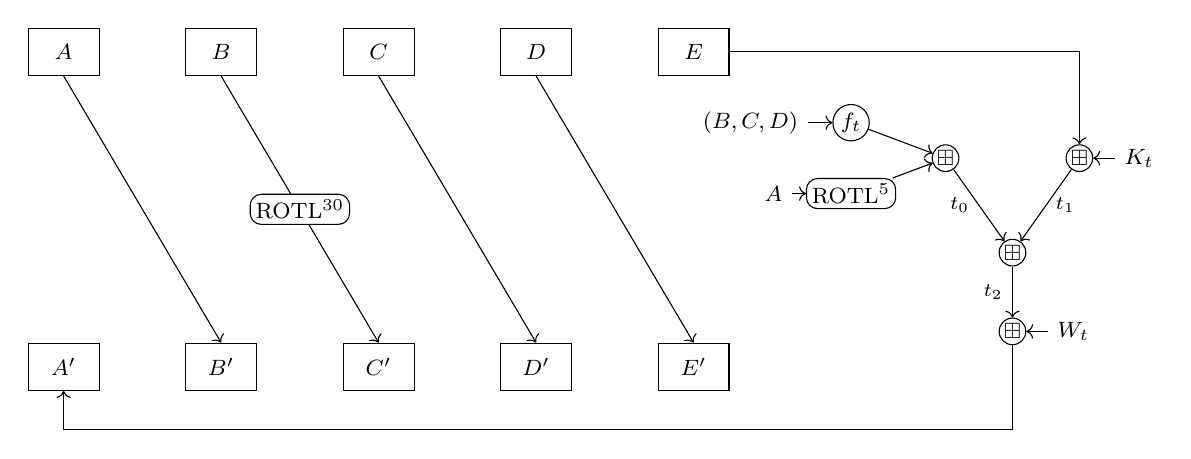
\begin{tikzpicture}[x=1cm,y=1cm,font=\footnotesize]
\foreach \n/\x in {A/0,B/2,C/4,D/6,E/8}{\node[draw,minimum width=0.9cm,minimum height=0.6cm] (\n) at (\x,4) {$\n$};}
\foreach \n/\l/\x in {A2/A'/0,B2/B'/2,C2/C'/4,D2/D'/6,E2/E'/8}{\node[draw,minimum width=0.9cm,minimum height=0.6cm] (\n) at (\x,0) {$\l$};}
\draw[->] (A.south) -- (B2.north);
\node[draw,rounded corners,inner sep=2pt,fill=white] (r30) at (3,2) {$\rotl{30}$};
\draw (B.south) -- (r30); \draw[->] (r30) -- (C2.north);
\draw[->] (C.south) -- (D2.north);
\draw[->] (D.south) -- (E2.north);
% balanced tree of four two-operand adders, as in the generator (add5)
\node[draw,circle,inner sep=1pt] (f) at (10.0,3.1) {$f_t$};
\node[anchor=east] (fin) at (9.45,3.1) {$(B,C,D)$};
\node[draw,rounded corners,inner sep=2pt] (r5) at (10.0,2.2) {$\rotl{5}$};
\node[anchor=east] (ain) at (9.25,2.2) {$A$};
\node[draw,circle,inner sep=0.5pt] (p1) at (11.2,2.65) {$\boxplus$};
\node[draw,circle,inner sep=0.5pt] (p2) at (12.9,2.65) {$\boxplus$};
\node[anchor=west] (K) at (13.35,2.65) {$K_t$};
\node[draw,circle,inner sep=0.5pt] (p3) at (12.05,1.45) {$\boxplus$};
\node[draw,circle,inner sep=0.5pt] (p4) at (12.05,0.45) {$\boxplus$};
\node[anchor=west] (W) at (12.5,0.45) {$W_t$};
\draw[->] (fin) -- (f); \draw[->] (f) -- (p1);
\draw[->] (ain) -- (r5); \draw[->] (r5) -- (p1);
\draw[->] (E.east) -| (p2.north);
\draw[->] (K) -- (p2);
\draw[->] (p1) -- node[font=\scriptsize,left]{$t_0$} (p3);
\draw[->] (p2) -- node[font=\scriptsize,right]{$t_1$} (p3);
\draw[->] (p3) -- node[font=\scriptsize,left]{$t_2$} (p4);
\draw[->] (W) -- (p4);
\draw[->] (p4.south) -- (12.05,-0.8) -| (A2.south);
\end{tikzpicture}
\caption{One SHA-1 round. The new $A$ is $\rotl{5}(A)\boxplus f_t(B,C,D)\boxplus E\boxplus K_t\boxplus W_t$;
the other words shift, with $B$ rotated by 30. The additions are drawn as the generator encodes them,
a balanced tree of four two-operand adders: $t_0=\rotl{5}(A)\boxplus f_t$, $t_1=E\boxplus K_t$,
$t_2=t_0\boxplus t_1$, and $A'=t_2\boxplus W_t$. Modular addition is associative, so the value is
independent of this arrangement, but the auxiliary variables, carries and clauses are not.}
\end{figure}

\paragraph{Reduced rounds and the preimage problem.} The $r$-round variant runs only rounds
$0,\dots,r-1$ and applies the feed-forward to the state at that point. A preimage instance fixes a
160-bit target digest and asks for any 512-bit block mapping to it, from the standard IV, under the
reduced-round compression function. The instances impose no message-padding constraints: all 512
block bits are free. A solution is therefore a preimage of one compression-function call, not
necessarily a correctly padded SHA-1 message. For a random target the expected
number of preimages is about $2^{512-160}=2^{352}$. The difficulty is finding one, not their
existence. Published cryptanalytic preimage attacks on reduced SHA-1 reach far more rounds than are
studied here, but only at costs far beyond any computation; the purpose here is to measure a
\emph{solver architecture} on a hard, standard, verifiable family, not to advance the attack frontier.

\subsection{Encoding as SAT}

Instances are produced by \texttt{sha1-sat} \cite{nossum}, with Tseitin-encoded adders
\cite{tseitin}. Every state, schedule and auxiliary bit is a Boolean variable, and every operation
becomes clauses:
\begin{itemize}
\item \textbf{Message schedule} (stage \texttt{EXPAND}): each bit of $W_t$, $t\ge16$, is the parity
of four bits, encoded directly as the 16 clauses of width 5 that forbid the odd assignments. No
auxiliary variables are needed.
\item \textbf{Rounds} (stage \texttt{ROUND}): $f_t$ is encoded per bit: six 3-literal clauses per bit
for $\mathrm{Ch}$, and the eight 4-literal parity clauses per bit for $\mathrm{Parity}$ (the 512
width-4 clauses of Table~\ref{tab:enc} are the two Parity rounds). The five-operand sum is a balanced
tree of four two-operand adders (Figure~1): $t_0=\rotl{5}(A)\boxplus f_t$, $t_1=E\boxplus K_t$,
$t_2=t_0\boxplus t_1$, and result $=t_2\boxplus W_t$. Each two-operand adder is built from Tseitin gates per bit: a half-sum
XOR, a generate AND, a propagate-and-carry AND, a carry OR, and a sum XOR. Rotations are free: they
only rename variables.
\item \textbf{Constants and IV} (\texttt{CONST}) and the \textbf{target digest} (\texttt{FIX}) are
unit clauses. The feed-forward adds (\texttt{FINAL}) are further Tseitin adders.
\end{itemize}

\begin{table}[h]\centering\small
\begin{tabular}{@{}lrrrrrrr@{}}
\toprule
$r$ & \textbf{variables} & \textbf{clauses} & \texttt{EXPAND} & \texttt{ROUND} & \texttt{FINAL} & \texttt{CONST} & \texttt{FIX}\\
\midrule
21 & 15{,}516 & 54{,}363 & 2{,}560 & 48{,}700 & 2{,}655 & 288 & 160\\
22 & 16{,}204 & 57{,}255 & 3{,}072 & 51{,}080 & 2{,}655 & 288 & 160\\
\bottomrule
\end{tabular}
\caption{Size of the encoding by stage. At $r=22$ the clause widths are: 448 units, 17{,}298
binary, 35{,}925 ternary, 512 of width 4 and 3{,}072 of width 5.}
\label{tab:enc}
\end{table}

Two practical details matter. First, the generator's DIMACS header overstates the clause count by
288: each 32-bit constant is counted once per word and again per bit. Dagster rejects such a file,
so the header is repaired. Second, the generator labels its variables in comment lines
(\texttt{w[i]}, \texttt{a[i]}, \texttt{carry}, $\dots$), which lets tools locate the message-block bits and
the state words. Verification uses these labels: it reads the 512 message-block bits from a model,
recomputes $r$-round SHA-1, and compares the digest with the target. With the option
\texttt{--xor} the generator instead emits every XOR relation as a native XOR constraint, the input
format that CryptoMiniSat's Gaussian elimination works on. That covers the sum bits of every adder,
the message schedule and the Parity rounds. At $r=21$ there are 5{,}799: 5{,}292 from the 84 round
adders, 315 from the five feed-forward adders, 160 from the schedule words $W_{16..20}$ and 32 from
the single Parity round, beside 29{,}119 ordinary clauses.

\subsection{SAT solving}

Conflict-driven clause learning (CDCL) solvers \cite{minisat} assign variables, propagate the
implied literals, and on a conflict derive a \emph{learnt clause} that blocks the conflict's cause,
then backtrack. Their progress is usually measured in conflicts. An \emph{incremental} solver keeps
its clause database and learnt clauses across calls; \emph{assumptions} fix literals for one call
only. Two standard parallel schemes are relevant:
\begin{itemize}
\item a \textbf{portfolio} runs independent solvers, diversified by random seeds, and stops at the
first answer;
\item \textbf{cube-and-conquer} splits the search space by fixing a few variables (a \emph{cube})
per subproblem.
\end{itemize}
CryptoMiniSat \cite{cms} extends CDCL with native XOR reasoning by Gaussian elimination, designed for
cryptographic instances like this one.

\subsection{Dagster}

Dagster \cite{burgess2022dagster,burgess2023dagster} solves a CNF by a DAG whose nodes are clause subsets. A node's satisfying
assignments, projected onto the variables of an outgoing edge, become \emph{messages} that condition
its successor. A node with several incoming edges is a \emph{join}: it combines compatible parent
messages. A model of a terminal node, together with the messages that led to it, is a solution of
the formula.

A master process (MPI rank 0) generates messages and dispatches them to worker ranks. Its buffer
holds at most one live message per worker. The features used here are:
\begin{itemize}
\item \flag{-b 0}: depth-first message generation (deepest node, then lowest index);
\item \flag{-m 4} with \flag{-q 2}: persistent per-node MiniSat solvers, with incoming traces passed
as assumptions;
\item \flag{-e 0}: stop at the first terminal solution; \flag{-e 2}: one solution per disjoint
subgraph;
\item \flag{-i 1}: workers poll the master after every emitted solution.
\end{itemize}
When a worker emits a solution, the master stores it as a no-good and \emph{refreshes} the other
workers on the same message with it, so that they do not rediscover it. A worker reports a message
finished (\texttt{REQUEST\_FOR\_ASSIGNMENT}) only when its solver finds no further solution.

\subsection{The road to the 22-round result}\label{sec:diagnosis}

This section summarises the diagnosis that preceded the work reported here. Full numbers are in the
project's earlier report.

\paragraph{Portfolio baseline and the round cliff.} A 63-worker TiniSAT portfolio (Dagster's default
engine, diversified by clause permutation) solved 500 of 500 trajectories at $r=20$ (median about
1.8\,s) but only 40 of 500 (8\%) at $r=21$, and none at $r=22$, within 300\,s. The per-round growth
in median conflicts was about $\times7$ up to $r=20$, then $\times41$--$192$ from $r=20$ to $r=21$.

\paragraph{Restriction hardness.} Fixing $k$ bits of a \emph{planted} (guaranteed satisfiable) cube
gave an easy--hard--easy profile at $r=20$: $k\le16$ easy, $k=32$--$448$ unresolved within 150k
conflicts, $k\ge480$ trivial. Intermediate restrictions are hard even when a solution exists. This
explained why cube-and-conquer, which solved 69 of 640 cubes at $r=21$, found nothing in 640 cubes
at $r=22$. The ``$r=22$ wall'' was an artefact of cube restriction.

\paragraph{Attribution of an apparent Dagster advantage.} An early Dagster run with 7-bit cubes beat
the realised portfolio race in 10 of 15 comparisons. A controlled study showed that the 63 dispatched
jobs were clause-identical to the standalone cube census, and that a dumped job reproduced the census
conflict count exactly. The apparent gain came from dispatch order and execution context: one
computation took 40\,s under full load against 20.6\,s alone. Methods are compared here only under
matched context.

\paragraph{Structural decomposition.} Exact max-flow gives minimum vertex separators of 320--448
variables between round blocks. Round-aligned cuts are already optimal, and the graph is path-like.
A round-boundary split-join did not filter: both halves accepted 200 of 200 random boundary
assignments, bounding the rejection rate below 1.49\% at 95\% confidence.

\paragraph{The trans-round trace relaxation.} Fixing the planted low-16 bits of every free state word
cut the solve from 866{,}048 to 14{,}609 conflicts ($\approx59\times$, Kissat, $r=21$). Low-8 gave only
$1.35\times$. Interior 8-bit slices, whose carry-in is unknown, made the problem \emph{harder}. Random
low-16 traces are refuted at once, so the trace space filters strongly. The relaxation $R_{16}$ is an
exact clause subset, sound by construction, and about 0.3--0.4\% of its traces extend at $r=21$. This
was the first interface in the project that filtered.

\paragraph{The 21-round demonstrator.} On the campaign workstation (64 physical cores) a compositional race and the low16
pipeline each solved 50 of 50 runs over five targets, with medians of about 4\,s, against realised
64-worker MiniSat races of 4.1--7.8\,s. At $r=21$ every arm is near a floor set mostly by Dagster's
roughly 3\,s start-up, so the round could not discriminate between them. The compositional race had
no slow tail: 0 of 50 runs over 10\,s.

\paragraph{The 22-round pilot and the refinement lock.} On one target (g10005):
\begin{itemize}
\item the portfolio solved 4 of 64 trajectories within 1800\,s, the fastest at 259\,s;
\item the low16 pipeline solved 5 of 5 runs (260--768\,s);
\item the compositional race solved one run in 15.4\,s, and four runs were ended as stalls.
\end{itemize}
The event logs located the cause (Figure~\ref{fig:lock}). The staged pipeline's refinement node
turns every extendable low-8 trace into a never-ending enumeration of low-16 refinements. These
messages never complete, so they fill the buffer, and every terminal job is created in the first
half-second. In the locked run shown, about 5{,}700 refined traces were produced and none was ever
checked.

\begin{figure}[h]\centering
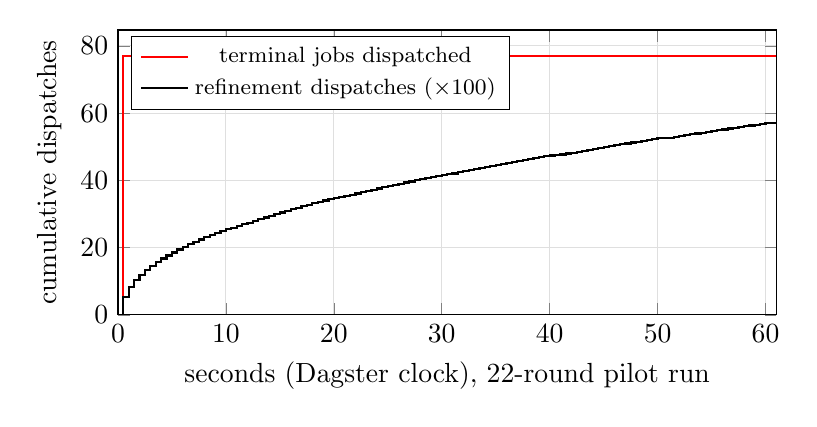
\begin{tikzpicture}
\begin{axis}[width=0.82\textwidth,height=5.2cm,xmin=0,xmax=61,ymin=0,
 xlabel={seconds (Dagster clock), 22-round pilot run},ylabel={cumulative dispatches},
 legend style={font=\footnotesize,at={(0.02,0.98)},anchor=north west},grid=major,grid style={gray!25}]
\addplot[red,thick,const plot] coordinates {(0.000,0.0000) (0.500,77.0000) (1.000,77.0000) (1.500,77.0000) (2.000,77.0000) (2.500,77.0000) (3.000,77.0000) (3.500,77.0000) (4.000,77.0000) (4.500,77.0000) (5.000,77.0000) (5.500,77.0000) (6.000,77.0000) (6.500,77.0000) (7.000,77.0000) (7.500,77.0000) (8.000,77.0000) (8.500,77.0000) (9.000,77.0000) (9.500,77.0000) (10.000,77.0000) (10.500,77.0000) (11.000,77.0000) (11.500,77.0000) (12.000,77.0000) (12.500,77.0000) (13.000,77.0000) (13.500,77.0000) (14.000,77.0000) (14.500,77.0000) (15.000,77.0000) (15.500,77.0000) (16.000,77.0000) (16.500,77.0000) (17.000,77.0000) (17.500,77.0000) (18.000,77.0000) (18.500,77.0000) (19.000,77.0000) (19.500,77.0000) (20.000,77.0000) (20.500,77.0000) (21.000,77.0000) (21.500,77.0000) (22.000,77.0000) (22.500,77.0000) (23.000,77.0000) (23.500,77.0000) (24.000,77.0000) (24.500,77.0000) (25.000,77.0000) (25.500,77.0000) (26.000,77.0000) (26.500,77.0000) (27.000,77.0000) (27.500,77.0000) (28.000,77.0000) (28.500,77.0000) (29.000,77.0000) (29.500,77.0000) (30.000,77.0000) (30.500,77.0000) (31.000,77.0000) (31.500,77.0000) (32.000,77.0000) (32.500,77.0000) (33.000,77.0000) (33.500,77.0000) (34.000,77.0000) (34.500,77.0000) (35.000,77.0000) (35.500,77.0000) (36.000,77.0000) (36.500,77.0000) (37.000,77.0000) (37.500,77.0000) (38.000,77.0000) (38.500,77.0000) (39.000,77.0000) (39.500,77.0000) (40.000,77.0000) (40.500,77.0000) (41.000,77.0000) (41.500,77.0000) (42.000,77.0000) (42.500,77.0000) (43.000,77.0000) (43.500,77.0000) (44.000,77.0000) (44.500,77.0000) (45.000,77.0000) (45.500,77.0000) (46.000,77.0000) (46.500,77.0000) (47.000,77.0000) (47.500,77.0000) (48.000,77.0000) (48.500,77.0000) (49.000,77.0000) (49.500,77.0000) (50.000,77.0000) (50.500,77.0000) (51.000,77.0000) (51.500,77.0000) (52.000,77.0000) (52.500,77.0000) (53.000,77.0000) (53.500,77.0000) (54.000,77.0000) (54.500,77.0000) (55.000,77.0000) (55.500,77.0000) (56.000,77.0000) (56.500,77.0000) (57.000,77.0000) (57.500,77.0000) (58.000,77.0000) (58.500,77.0000) (59.000,77.0000) (59.500,77.0000) (60.000,77.0000) (60.500,77.0000) (61.000,77.0000)};\addlegendentry{terminal jobs dispatched}
\addplot[black,thick,const plot] coordinates {(0.000,0.0000) (0.500,5.3100) (1.000,8.2600) (1.500,10.3400) (2.000,11.9800) (2.500,13.4000) (3.000,14.6400) (3.500,15.7700) (4.000,16.7600) (4.500,17.6800) (5.000,18.5800) (5.500,19.4300) (6.000,20.2400) (6.500,20.9700) (7.000,21.7000) (7.500,22.4100) (8.000,23.0900) (8.500,23.7400) (9.000,24.3700) (9.500,24.9500) (10.000,25.5400) (10.500,25.8100) (11.000,26.3800) (11.500,26.9400) (12.000,27.4300) (12.500,27.9600) (13.000,28.4800) (13.500,28.9900) (14.000,29.4900) (14.500,29.9900) (15.000,30.4500) (15.500,30.9300) (16.000,31.3900) (16.500,31.8400) (17.000,32.2900) (17.500,32.7400) (18.000,33.1800) (18.500,33.6100) (19.000,34.0400) (19.500,34.4500) (20.000,34.8400) (20.500,34.9400) (21.000,35.3300) (21.500,35.7200) (22.000,36.0800) (22.500,36.4700) (23.000,36.8400) (23.500,37.1900) (24.000,37.5500) (24.500,37.9200) (25.000,38.2800) (25.500,38.6300) (26.000,38.9900) (26.500,39.3400) (27.000,39.6900) (27.500,40.0400) (28.000,40.3900) (28.500,40.7300) (29.000,41.0600) (29.500,41.3900) (30.000,41.7100) (30.500,41.8100) (31.000,42.0500) (31.500,42.3700) (32.000,42.6700) (32.500,42.9800) (33.000,43.2900) (33.500,43.6000) (34.000,43.9100) (34.500,44.2100) (35.000,44.5100) (35.500,44.8200) (36.000,45.1100) (36.500,45.3900) (37.000,45.6900) (37.500,45.9800) (38.000,46.2700) (38.500,46.5600) (39.000,46.8500) (39.500,47.1300) (40.000,47.4200) (40.500,47.5200) (41.000,47.6900) (41.500,47.9700) (42.000,48.2500) (42.500,48.5300) (43.000,48.8100) (43.500,49.0800) (44.000,49.3600) (44.500,49.6300) (45.000,49.9000) (45.500,50.1700) (46.000,50.4400) (46.500,50.7100) (47.000,50.9600) (47.500,51.2300) (48.000,51.4900) (48.500,51.7400) (49.000,51.9900) (49.500,52.2400) (50.000,52.4900) (50.500,52.6000) (51.000,52.7100) (51.500,52.9500) (52.000,53.2000) (52.500,53.4500) (53.000,53.7000) (53.500,53.9400) (54.000,54.1900) (54.500,54.4300) (55.000,54.6800) (55.500,54.9200) (56.000,55.1500) (56.500,55.3900) (57.000,55.6200) (57.500,55.8600) (58.000,56.1000) (58.500,56.3300) (59.000,56.5600) (59.500,56.7900) (60.000,57.0300) (60.500,57.1400) (61.000,57.2100)};\addlegendentry{refinement dispatches ($\times100$)}
\end{axis}
\end{tikzpicture}
\caption{Anatomy of the refinement lock, in an unpatched 22-round pilot run. All 77 terminal jobs
were dispatched within 0.43\,s. The refinement node then produced about 95 refined traces per
second, none of which reached a terminal.}
\label{fig:lock}
\end{figure}

\subsection{Performance against CryptoMiniSat and other single solvers}\label{sec:cms}

None of the project's workstation campaigns used CryptoMiniSat, so it was measured for this report on a
separate machine (one core). CryptoMiniSat~5 (pycryptosat 5.17) ran on both the plain CNF and the
native-XOR encoding, beside MiniSat~2.2 (the solver family inside Dagster's mode~4) and CaDiCaL~1.9.5.
All solvers ran single-threaded with default settings, one seed, on the same instances, and each
model was verified (the verifier was extended to skip XOR lines, which it does not need, since it
recomputes SHA-1 from the message-block bits). Times on this machine are not comparable in absolute terms with the workstation's, and one
seed per cell measures a single trajectory of a heavy-tailed process, so the table is indicative
only.

\begin{table}[h]\centering\small
\begin{tabular}{@{}llrrl@{}}
\toprule
\textbf{instance} & \textbf{solver (encoding)} & \textbf{cap (s)} & \textbf{wall (s)} & \textbf{outcome}\\
\midrule
21 rounds, g10003 & MiniSat 2.2 (CNF) & 600 & 289.5 & solved, verified\\
21 rounds, g10003 & CaDiCaL 1.9.5 (CNF) & 400 & 134.1 & solved, verified\\
21 rounds, g10003 & CryptoMiniSat 5 (CNF) & 400 & 30.1 & solved, verified\\
21 rounds, g10003 & CryptoMiniSat 5 (native XOR) & 400 & 61.5 & solved, verified\\
22 rounds, g10005 & CryptoMiniSat 5 (native XOR) & 900 & --- & not solved\\
22 rounds, g10005 & CryptoMiniSat 5 (CNF) & 900 & 396.6 & solved, verified\\
\bottomrule
\end{tabular}
\caption{Single-thread solvers on one core (not the campaign workstation). ``Solved'' means a verified preimage within
the cap.}
\label{tab:cms}
\end{table}

For context on the campaign workstation, the relevant single-solver reference is the trajectory census of MiniSat with
random initialisation:
\begin{itemize}
\item at $r=21$, 248 of 320 trajectories (78\%) were verified within 300\,s, with a median of 154\,s;
\item at $r=22$ (Phase C), only 2 of 64 trajectories per target solved within 1800\,s.
\end{itemize}
A brief earlier probe on the workstation also ran Kissat, which solved one 21-round target in 47\,s (866k
conflicts) against 151\,s for CaDiCaL, but did not solve a 22-round target within 265\,s.

On this machine CryptoMiniSat on the plain CNF was the fastest single solver at 21 rounds: 30.1\,s,
against 134.1\,s for CaDiCaL and 289.5\,s for MiniSat, about ten times MiniSat. Its native-XOR
encoding was slower (61.5\,s), so the advantage did not come from Gaussian elimination. At 22 rounds
CryptoMiniSat on the plain CNF found a verified preimage in 396.6\,s on one core, while the XOR
encoding did not finish within 900\,s.

This single trajectory is striking against the workstation MiniSat census, where only about 3\% of
trajectories solved a 22-round target within 1800\,s. It is one seed on one instance and one machine,
a single draw from a heavy-tailed distribution, so it ranks nothing. It does mean that the advantage
reported in this study is relative to a \emph{MiniSat} portfolio; a portfolio of a stronger solver is
a materially stronger baseline (open item R5).

%=============================================================================================
\section{Summary of results}
The terms used here are defined in Section~\ref{sec:background}, in particular
Section~\ref{sec:notation}.
%=============================================================================================

\paragraph{Problem.} Given a 160-bit digest of $r$-round SHA-1, find a 512-bit message block that
produces it. The instance is a CNF formula of about $1.6\times10^4$ variables and
$5.7\times10^4$ clauses at $r=22$. Every model found is checked by recomputing SHA-1, independently
of any solver.

\paragraph{Approach.} A Dagster DAG races several pipelines whose nodes refer to clause subsets of
one combined CNF file. Each node's worker-local incremental solver keeps its own learned clauses;
there is no global exchange of learned clauses between components. Each
pipeline first solves a \emph{relaxation} $R_k$ (the clauses for the low $k$ bits of every adder),
projects its model onto a trace $z_k$, and passes the trace to a terminal node holding the exact
formula, which extends it or refutes it. A \emph{staged} pipeline refines low-8 traces to low-16
before the exact check.

\paragraph{Obstacle and fix.} At 22 rounds the staged pipeline's refinement node never completes a
message, so all terminal work stops within the first second (Section~\ref{sec:diagnosis}). The patch
(Section~\ref{sec:method}) adds a refinement retirement threshold $L$: a worker that has emitted $L$
descendants for a parent message asks the master to retire it.

\paragraph{Evidence.}
\begin{center}\small
\begin{tabular}{@{}lccc@{}}
\toprule
\textbf{Locked evaluation, 22 rounds, 3 untouched targets} & \textbf{solved} & \textbf{median} & \textbf{ver./phys.\ core-h}\\
\midrule
Compositional race, $L=8$ & 30/30 & 26.9\,s & 1.38\\
low16 pipeline alone & 30/30 & 40.8\,s & 0.60\\
Observed 64-core MiniSat portfolio race & 28/30 & 553\,s & 0.07\\
\bottomrule
\end{tabular}
\end{center}
The compositional race was faster than the portfolio race in 30 of 30 pairs, and 10 of 10 on each
target. Against the low16 pipeline alone it won 16 of 30 pairs ($p=0.86$). Both solved all 30 runs,
so the evidence supports robustness in \emph{run time} (the full race stays fast on every target,
whereas low16 alone is much slower on g10003) and higher yield, not a difference in solved fraction. The conflict budgets
were measured to be harmful at this scale and were disabled for the evaluation.

\paragraph{Scope of the comparison.} Both arms use the same solver, MiniSat~2.2. A separate
single-core measurement found CryptoMiniSat about ten times faster than MiniSat on a 21-round
instance, and one CryptoMiniSat trajectory solved a 22-round target in 397\,s
(Section~\ref{sec:cms}). The result is therefore a statement about decomposition relative to a
MiniSat portfolio. Whether it holds against a portfolio of a stronger solver, or with a stronger
solver inside Dagster's workers, is the most important open question (R5).

%=============================================================================================
\section{DAG designs explored}\label{sec:dags}
%=============================================================================================

The notation for node contents is:
\begin{itemize}
\item $F$, the full exact formula (all original clauses, including the digest units);
\item $R_k$, the relaxation (Table~\ref{tab:relax}): all \texttt{CONST}, \texttt{EXPAND} and
\texttt{FIX} clauses, plus every \texttt{ROUND}/\texttt{FINAL} adder and $f_t$ clause whose bit
position is below $k$;
\item $z_k$, the trace: bits $0..k-1$ of every free state word $a_5,\dots,a_{r-1}$, which is
$(r-5)k$ bits, so 272 bits for $k=16$ at $r=22$;
\item $D_{ij}$, two unit clauses fixing bit 0 of $w_0$ to $i$ and bit 0 of $w_1$ to $j$;
\item $c_{15}$, the carry out of bit 15 of every adder chain.
\end{itemize}
Each edge is labelled with the variables its messages assign.

\begin{table}[h]\centering\small
\begin{tabular}{@{}lrrrr@{}}
\toprule
 & $R_8$ & $R_{12}$ & $R_{16}$ & $R_{20}$\\
\midrule
clauses (of 57{,}255) & 16{,}838 & 23{,}706 & 30{,}574 & 37{,}442\\
trace bits $|z_k|$ & 136 & 204 & 272 & 340\\
\bottomrule
\end{tabular}
\caption{Relaxation sizes at $r=22$.}
\label{tab:relax}
\end{table}

\begin{figure}[p]\centering
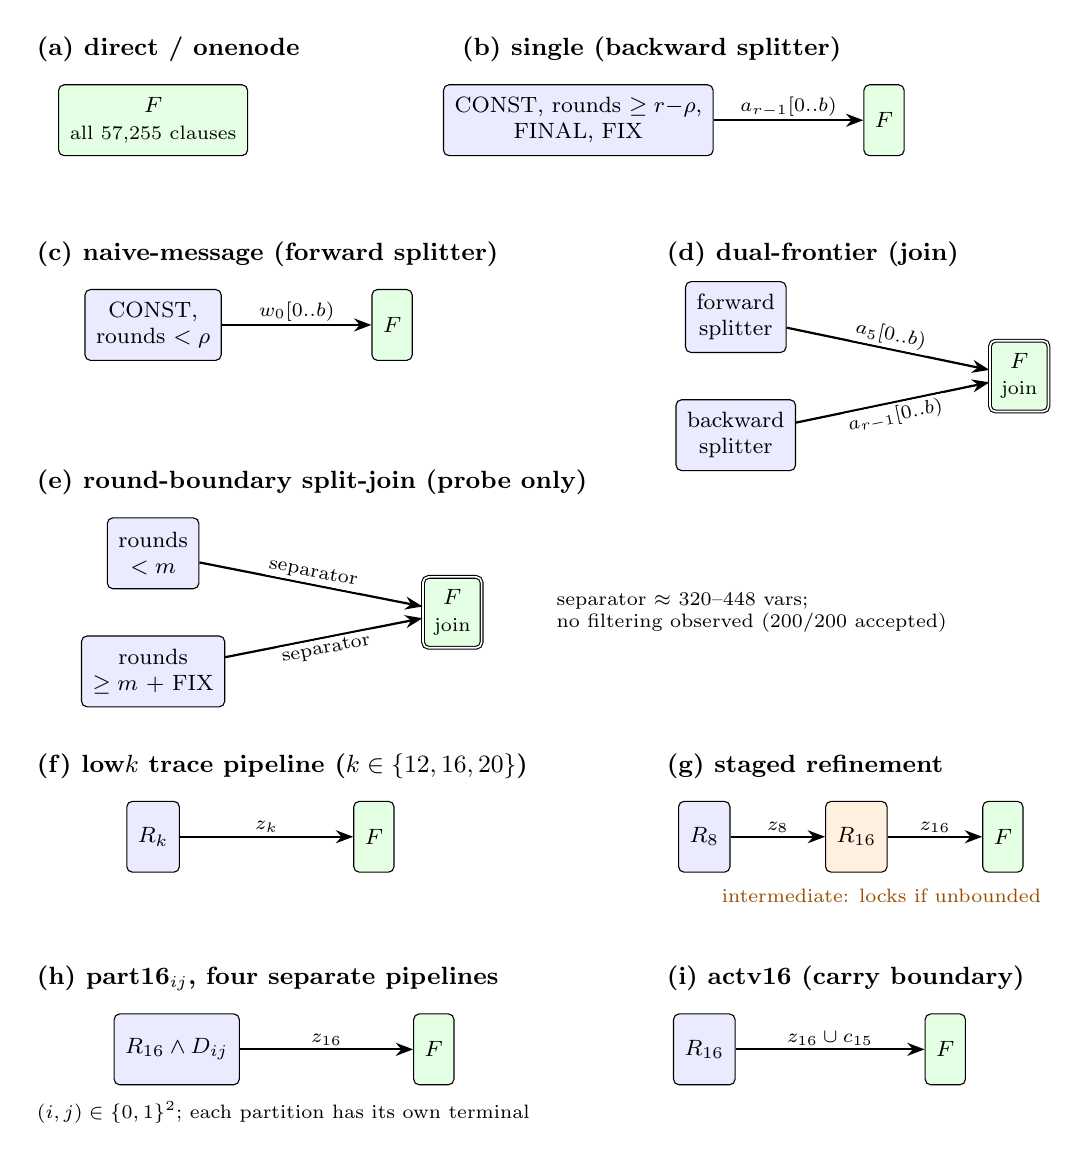
\begin{tikzpicture}[node distance=1.15cm and 1.5cm]
% (a) direct
\node[font=\small\bfseries,anchor=west] at (-1,0.9) {(a) direct / onenode};
\node[term,minimum width=2.4cm] (a1) at (0.6,0) {$F$\\ \scriptsize all 57{,}255 clauses};
% (b) single
\node[font=\small\bfseries,anchor=west] at (4.4,0.9) {(b) single (backward splitter)};
\node[src] (b1) at (6.0,0) {CONST, rounds $\ge r{-}\rho$,\\FINAL, FIX};
\node[term,right=1.9cm of b1] (b2) {$F$};
\draw[ed] (b1) -- node[el,above]{$a_{r-1}[0..b)$} (b2);
% (c) naive
\node[font=\small\bfseries,anchor=west] at (-1,-1.7) {(c) naive-message (forward splitter)};
\node[src] (c1) at (0.6,-2.6) {CONST,\\ rounds $<\rho$};
\node[term,right=1.9cm of c1] (c2) {$F$};
\draw[ed] (c1) -- node[el,above]{$w_0[0..b)$} (c2);
% (d) dual frontier (join)
\node[font=\small\bfseries,anchor=west] at (7.0,-1.7) {(d) dual-frontier (join)};
\node[src] (d1) at (8.0,-2.5) {forward\\ splitter};
\node[src] (d2) at (8.0,-4.0) {backward\\ splitter};
\node[joinnd] (d3) at (11.6,-3.25) {$F$\\\scriptsize join};
\draw[ed] (d1) -- node[el,above,sloped]{$a_5[0..b)$} (d3);
\draw[ed] (d2) -- node[el,below,sloped]{$a_{r-1}[0..b)$} (d3);
% (e) split-join probe
\node[font=\small\bfseries,anchor=west] at (-1,-4.6) {(e) round-boundary split-join (probe only)};
\node[src] (e1) at (0.6,-5.5) {rounds\\ $<m$};
\node[src] (e2) at (0.6,-7.0) {rounds\\ $\ge m$ + FIX};
\node[joinnd] (e3) at (4.4,-6.25) {$F$\\\scriptsize join};
\draw[ed] (e1) -- node[el,above,sloped]{separator} (e3);
\draw[ed] (e2) -- node[el,below,sloped]{separator} (e3);
\node[font=\scriptsize,align=left,anchor=west] at (5.6,-6.25) {separator $\approx$ 320--448 vars;\\ no filtering observed (200/200 accepted)};
% (f) low-k
\node[font=\small\bfseries,anchor=west] at (-1,-8.2) {(f) low$k$ trace pipeline ($k\in\{12,16,20\}$)};
\node[src] (f1) at (0.6,-9.1) {$R_k$};
\node[term,right=2.2cm of f1] (f2) {$F$};
\draw[ed] (f1) -- node[el,above]{$z_k$} (f2);
% (g) staged
\node[font=\small\bfseries,anchor=west] at (7.0,-8.2) {(g) staged refinement};
\node[src] (g1) at (7.6,-9.1) {$R_8$};
\node[ref,right=1.2cm of g1] (g2) {$R_{16}$};
\node[term,right=1.2cm of g2] (g3) {$F$};
\draw[ed] (g1) -- node[el,above]{$z_8$} (g2);
\draw[ed] (g2) -- node[el,above]{$z_{16}$} (g3);
\node[font=\scriptsize,text=orange!60!black] at (9.85,-9.85) {intermediate: locks if unbounded};
% (h) part16
\node[font=\small\bfseries,anchor=west] at (-1,-10.9) {(h) part16$_{ij}$, four separate pipelines};
\node[src] (h1) at (0.9,-11.8) {$R_{16}\wedge D_{ij}$};
\node[term,right=2.2cm of h1] (h2) {$F$};
\draw[ed] (h1) -- node[el,above]{$z_{16}$} (h2);
\node[font=\scriptsize,anchor=west] at (-1,-12.6) {$(i,j)\in\{0,1\}^2$; each partition has its own terminal};
% (i) actv16
\node[font=\small\bfseries,anchor=west] at (7.0,-10.9) {(i) actv16 (carry boundary)};
\node[src] (i1) at (7.6,-11.8) {$R_{16}$};
\node[term,right=2.4cm of i1] (i2) {$F$};
\draw[ed] (i1) -- node[el,above]{$z_{16}\cup c_{15}$} (i2);
\end{tikzpicture}
\caption{Every DAG family explored, with node contents. Blue: source (root) nodes. Orange: the
intermediate refinement node. Green: terminals holding the exact formula $F$; a doubled border marks
a join. (b)--(d) are the cube-and-conquer DAGs of the attribution study (splitters cover $\rho$
rounds; edges carry $b$-bit cubes). (e) was evaluated as a filtering probe only. (f)--(i) are the
trace-relaxation components. Every terminal contains all of $F$, so any reported model satisfies the
original formula.}
\label{fig:dags}
\end{figure}

\begin{figure}[h]\centering
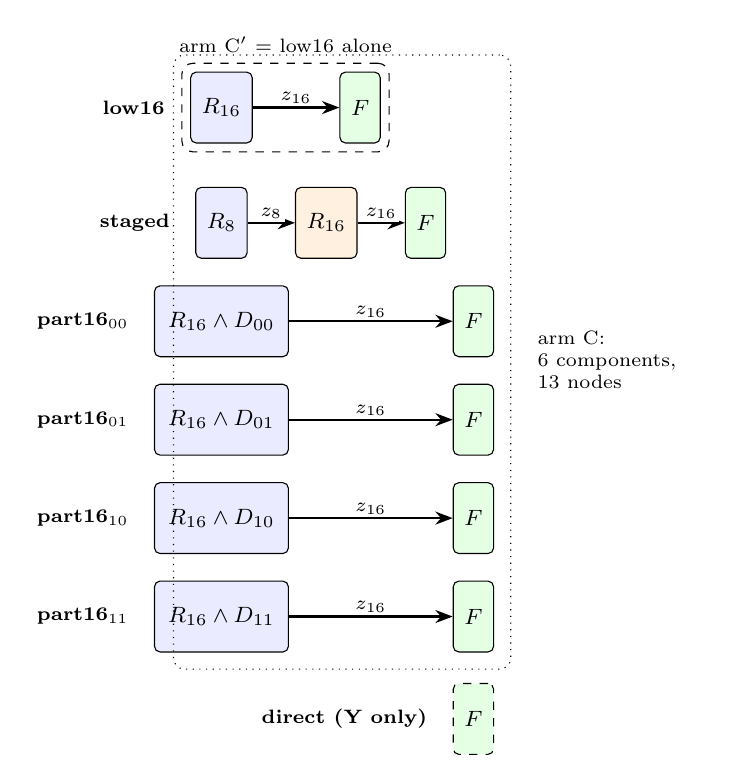
\begin{tikzpicture}[node distance=0.55cm and 1.1cm]
\node[src] (l1) {$R_{16}$}; \node[term,right=of l1] (l2) {$F$}; \draw[ed] (l1) -- node[el,above]{$z_{16}$} (l2);
\node[font=\scriptsize\bfseries,left=0.2cm of l1] {low16};
\node[src,below=of l1] (s1) {$R_8$}; \node[ref,right=0.6cm of s1] (s2) {$R_{16}$}; \node[term,right=0.6cm of s2] (s3) {$F$};
\draw[ed] (s1) -- node[el,above]{$z_8$} (s2); \draw[ed] (s2) -- node[el,above]{$z_{16}$} (s3);
\node[font=\scriptsize\bfseries,left=0.2cm of s1] {staged};
\foreach \i/\j/\k in {0/0/1,0/1/2,1/0/3,1/1/4}{
  \node[src,minimum width=1.7cm] (p\k) at ($(s1)+(0,-1.25*\k)$) {$R_{16}\wedge D_{\i\j}$};
  \node[term] (q\k) at ($(p\k)+(3.2,0)$) {$F$};
  \draw[ed] (p\k) -- node[el,above]{$z_{16}$} (q\k);
  \node[font=\scriptsize\bfseries,left=0.2cm of p\k] {part16$_{\i\j}$};}
\node[term,dashed] (dd) at ($(q4)+(0,-1.3)$) {$F$};
\node[font=\scriptsize\bfseries,left=0.2cm of dd] {direct (Y only)};
\node[draw,dotted,rounded corners,inner sep=6pt,fit=(l1)(l2)(s3)(q4),label={[font=\scriptsize]right:\begin{tabular}{l}arm C:\\6 components,\\13 nodes\end{tabular}}] {};
\node[draw,dashed,rounded corners,inner sep=3pt,fit=(l1)(l2),label={[font=\scriptsize]above:arm C$'$ = low16 alone}] {};
\end{tikzpicture}
\caption{The DAGs of the evaluation, whose nodes all draw clause subsets from one combined CNF. Arm C contains six disjoint
components (13 nodes) racing under \flag{-e 0}; the first verified terminal solution ends the run.
Arm C$'$ is the low16 component alone. The yield arm Y adds the direct component and runs under
\flag{-e 2}. The 21-round demonstrator also included low12, low20 and actv16.}
\label{fig:evaldag}
\end{figure}

%=============================================================================================
\section{Method: the refinement-retirement patch}\label{sec:method}
%=============================================================================================

\subsection{Where the lock comes from in the code}

Three properties of stock Dagster combine to cause the lock.
\begin{enumerate}
\item \textbf{A message ends only when its enumeration ends.} In the worker loop
(\texttt{Worker::loop}), after emitting a solution the worker calls
\texttt{reset\_solver\_for\_next\_solution}, which adds a blocking clause and asks for the next model.
It sends \texttt{MPI\_TAG\_REQUEST\_FOR\_ASSIGNMENT} (``this message is finished'') only when that
call reports no further model, or under \flag{-e 3}. The staged refinement node $R_{16}$ conditioned
on an extendable $z_8$ has an astronomically large model set, so the message effectively never ends.
\item \textbf{The buffer is finite.} The master keeps at most one live message per worker. Root
enumerations hold slots permanently by design. Extendable refinement messages accumulate until they
occupy the rest.
\item \textbf{Mode-4 workers cannot yield.} A MiniSat call (\texttt{MinisatSolver::run}) runs to
completion, so a worker on a long terminal check cannot be pre-empted; stock Dagster's \flag{-j}
decision limit applies only to its TiniSAT modes.
\end{enumerate}
With \flag{-b 0} the master would send freed slots straight to the deepest node, the staged terminal,
but no slot is ever freed. The patch therefore changes when an intermediate message ends, and adds an
optional way for MiniSat calls to yield.

\subsection{Design requirements}

The patch had to meet five requirements.
\begin{enumerate}
\item \textbf{Opt-in and inert.} With every control unset or zero it must preserve stock search and
scheduling semantics.
\item \textbf{Minimal.} Only \texttt{Worker.cpp} and \texttt{minisat\_solver/minisat\_solver.cc}
change; the master, the DAG format and the protocol are untouched.
\item \textbf{Sound.} No control may cause an incorrect model to be reported.
\item \textbf{Observable.} Every control action is logged with enough context to measure what it did.
\item \textbf{Fail-safe.} Invalid settings stop the run rather than silently doing something else.
\end{enumerate}

\subsection{Control 1: the refinement retirement threshold \texorpdfstring{$L$}{L}}

\paragraph{Classifying nodes.} The worker classifies the node it is solving from the DAG. Dagster
marks roots internally by giving them a \emph{self-loop} reverse connection: \texttt{Dag.cpp} sets
\texttt{reverse\_connections[i] = \{i\}} for every node without parents. A first version of the patch
tested ``has a reverse connection'' and so misclassified sources as intermediate nodes. It retired the
staged \emph{source} after one solution, and Dagster then correctly concluded that no work remained.
The final test is
\[
\textsf{is\_root}(n)\iff \textsf{rev}(n)=\{n\},\qquad
\textsf{intermediate}(n)\iff\neg\textsf{is\_root}(n)\wedge \textsf{fwd}(n)\neq\emptyset .
\]
The budget role is chosen in the same order: root first, then terminal, then intermediate. An
isolated node, such as the \emph{direct} component, is therefore treated as a \emph{source} for
budgeting. This had no effect here, because all budgets were zero in the evaluation and the direct
component appears only in the yield arm.

\paragraph{Counting per message.} The stock counter \texttt{solution\_count} is reset at every poll,
and with \flag{-i 1} a worker polls after every solution, so it never exceeds one. The patch keeps a
separate count \texttt{msg\_solutions}. Its key is the pair (node, assignment literals) of the current
message. The count is reset only when a message with a \emph{different} key is loaded, because the
master's refresh re-sends the \emph{same} message to the other workers whenever any of them emits.
In the locked pilot that happened about 5{,}700 times per run, and a count reset on every
re-delivery would never reach its threshold.

\paragraph{Retiring.} After each emitted solution on an intermediate node, if
$\texttt{msg\_solutions}\ge L$, the worker sends \texttt{REQUEST\_FOR\_ASSIGNMENT} in place of
continuing. On the master this calls \texttt{remove\_message}, which removes the message from the
buffer, frees \emph{every} worker allocated to it, and records the parent combination as completed,
so it is never regenerated. One worker's request therefore retires the parent for all. Each
retirement is logged:
\texttt{REFINEMENT\_RETIRE node=\dots\ msg=\dots\ emitted\_by\_this\_worker=\dots}.

\paragraph{Semantics.} The threshold is cooperative and worker-local, not a strict global bound.
Concurrent workers on the same parent keep private counts and can emit further descendants before
the master's removal reaches them. With $W$ workers on a parent the realised number of descendants
$N$ satisfies $L\le N\lesssim W L$. In practice it was measured, not assumed: at $L=8$ the maximum
was 9 in the regression and 10 over the 20 Step~3 control runs.

\begin{proposition}[Soundness]
With any setting of the controls, every reported model satisfies $F$.
\end{proposition}
\begin{proof}[Argument]
Retirement only removes messages and adds no clauses or literals, and each terminal holds all of $F$.
A terminal model satisfies $F$ by construction, and every model is independently verified in any case.
\end{proof}

\begin{proposition}[Incompleteness of finite \texorpdfstring{$L$}{L}]
For finite $L$ the staged component is incomplete: if the only extendable low-16 refinements of a
parent $z_8$ occur after the first $L$ emissions in the solver's order, they are never examined.
\end{proposition}
The low16 and part16 sources are not subject to the retirement threshold and can continue
generating alternatives while a run remains active. This prevents the retirement rule from imposing
the same finite per-parent cutoff on every component, but it does not make a finite, first-solution
run complete: runs stop at the first verified solution or at the 1800\,s cap, a source can generate
a vast stream of traces, and scheduling may prevent exhaustive enumeration.

\begin{center}\fbox{\parbox{0.9\textwidth}{\small\textbf{Sound but incomplete.} Retirement can prevent
Dagster from examining an otherwise successful refinement, but it cannot cause an invalid preimage to
be accepted. It changes \emph{which candidates are searched}, not the exact constraints used to
validate a terminal model.}}\end{center}

\subsection{Control 2: role-specific MiniSat conflict quanta}

The patch also lets a MiniSat call yield. Four environment variables set a conflict budget per node
role:
\begin{center}\footnotesize
\begin{tabular}{@{}ll@{}}
\toprule
\texttt{DAGSTER\_MINISAT\_TERMINAL\_CONFLICT\_BUDGET} & terminal nodes (no outgoing edges)\\
\texttt{DAGSTER\_MINISAT\_INTERMEDIATE\_CONFLICT\_BUDGET} & non-root nodes with outgoing edges\\
\texttt{DAGSTER\_MINISAT\_SOURCE\_CONFLICT\_BUDGET} & root nodes\\
\texttt{DAGSTER\_MINISAT\_CONFLICT\_QUANTUM} & default for any role not set\\
\bottomrule
\end{tabular}
\end{center}
Before each call the worker sets the budget for the node's role. If it is positive,
\texttt{MinisatSolver::run} calls \texttt{setConfBudget($N$)} (a limit relative to the current
conflict count, so each call gets a fresh quantum), then \texttt{solveLimited}, then
\texttt{budgetOff()}. It maps \texttt{l\_Undef} to Dagster's status~2, which triggers the existing
poll: the master may continue the job or reassign the worker.

A later quantum \emph{re-enters} the same assumption-conditioned problem in the persistent solver,
keeping learnt clauses and heuristic state. It does not continue the interrupted search stack.
Because status~2 also means ``poll for reassignment'' in other circumstances, budget exhaustion is
logged explicitly (\texttt{MINISAT\_BUDGET\_EXHAUSTED}). Every call's outcome and conflict use are
logged at verbosity~3 (\texttt{MINISAT\_RESULT}), which supplies the conflict distributions used for
calibration. Phase~B showed that this control is unnecessary, and harmful, at the scale studied
(Section~\ref{sec:phaseB}); it was disabled for the evaluation.

\subsection{Validation, observability and provenance}

At start-up each worker parses every control with \texttt{strtoll}. A non-integer, a negative value,
or a value above $10^{12}$ is fatal (\texttt{LOG(FATAL)}). The worker then logs one line,
\texttt{DAGSTER\_PATCH v3 L=\dots\ budget\_terminal=\dots\ budget\_intermediate=\dots\
budget\_source=\dots}, and the runsheets require the exact line before trusting a run (exit~9
otherwise). The patcher refuses an already-patched tree, keeps stock copies outside the build's
object globs, and writes the unified diff together with a manifest of SHA-256 hashes. The same diff
was used in all three phases:
\begin{center}\small
\begin{tabular}{@{}ll@{}}
\toprule
diff (unified, 135 lines) & \texttt{173dbcec\dots c6636892}\\
\texttt{Worker.cpp} stock $\to$ patched & \texttt{ba541d74\dots} $\to$ \texttt{20c747e8\dots}\\
\texttt{minisat\_solver.cc} stock $\to$ patched & \texttt{e6461ff8\dots} $\to$ \texttt{1c9267be\dots}\\
patch script & \texttt{68549a28\dots}\\
\bottomrule
\end{tabular}
\end{center}

\subsection{The patch in outline}

The behaviour of both controls, in pseudocode. The complete diff is in Appendix~\ref{app:patch}.
{\footnotesize\begin{verbatim}
at worker start:
    L, budget[source|intermediate|terminal] <- parse environment   (invalid value: fatal)
    log "DAGSTER_PATCH v3 L=... budget_terminal=... ..."
on loading a Dagster message m for node n:
    key <- (n, assignment literals of m)
    if key != current_key: current_key <- key; count <- 0   (a refresh keeps the count)
before each MiniSat call on node n:
    role <- source       if rev(n) = {n}            (Dagster's self-loop root marker)
            terminal     else if fwd(n) is empty
            intermediate otherwise
    result <- solve with conflict budget[role]       (0 = unlimited; 2 = exhausted -> poll)
after each solution emitted on node n:
    count <- count + 1
    if role = intermediate and L > 0 and count >= L:
        log REFINEMENT_RETIRE; send REQUEST_FOR_ASSIGNMENT  (master removes the parent)
\end{verbatim}}

\subsection{Supporting changes to the measurement harness}

The evaluation also depended on six changes outside Dagster.
\begin{itemize}
\item \textbf{Watcher.} A process tails the per-rank logs and verifies the first terminal solution
before ending the job. It flags a stall only when there is no new terminal dispatch \emph{and} no
terminal job is in flight. The earlier rule ended live checks: under the new rule $L=\infty$ solved
7 of 10 runs on the pilot target where the old one had stalled 4 of 5.
\item \textbf{Session-scoped cleanup.} Each run's session is cleaned up individually; there is no
global \texttt{pkill}.
\item \textbf{Launch checks.} A run fails closed (exit~8) if Dagster's master logs nothing.
\item \textbf{Log parsing.} All parsers skip glog's \texttt{<program>.INFO} symlink, which had made
one rank's lines count twice. This affected at most 1\% of events, and no dispatch records.
\item \textbf{Observed race runner.} The portfolio baseline arm (Br) is run as an observed race.
\item \textbf{Profiler.} A profiler reports realised descendants per parent and conflict quantiles.
\end{itemize}

%=============================================================================================
\section{Experimental protocol}\label{sec:protocol}
%=============================================================================================

\paragraph{Platform and resource accounting.} All runs used one machine, a 64-core AMD Ryzen Threadripper 3990X workstation (the \emph{campaign workstation}). Table~\ref{tab:res}
records what the run manifests captured, and states explicitly what they did not. (An earlier draft
gave an MPICH version of 4.0.2. That number came from a stand-in launcher used for testing, not from the workstation, and is withdrawn.)

\begin{table}[h]\centering\small
\begin{tabularx}{\textwidth}{@{}lL@{}}
\toprule
\textbf{Item} & \textbf{Value}\\
\midrule
CPU & AMD Ryzen Threadripper 3990X; one socket, one NUMA node; 256\,MiB L3 cache. Not recorded by the harness: taken with \texttt{lscpu} on the same machine after the campaign\\
Logical CPUs; SMT & 128; simultaneous multithreading active (two threads per core)\\
Physical cores & 64 (one socket of 64 cores, two hardware threads per core)\\
Kernel & Linux 5.4.0-148-generic\\
MPI & MPICH with the Hydra process manager; version not recorded\\
Dagster placement & \texttt{mpirun -bind-to core -n 65}: rank 0 (master) and 64 workers. With 65 ranks
on 64 cores at least two ranks share a physical core; under Hydra's cyclic core assignment this is
expected to be the master and one worker, but the placement was not recorded\\
Portfolio placement & 64 trajectories pinned with \texttt{taskset} to logical CPUs 0--63. On this
machine logical CPU $i$ is the first hardware thread of physical core $i$ for $i<64$, and CPUs 64--127
are the second threads of cores 0--63 (\texttt{lscpu -e=CPU,CORE}, taken after the campaign). The
portfolio therefore ran exactly one trajectory per physical core, with each core's second thread
idle\\
Core-hour denominator & \emph{Allocated physical core-hours}: 64 cores $\times$ wall time for every
arm. Yields in an earlier draft used 65 rank-hours for Dagster, which differs by $65/64$\\
\bottomrule
\end{tabularx}
\caption{Resources and accounting for every run on the campaign workstation.}
\label{tab:res}
\end{table}

Dagster ran with 65 ranks (64 workers and the master) and the flags \flag{-m 4 -q 2 -b 0 -i 1}. The
rounds were $r=22$, the cap was 1800\,s, and one experiment ran at a time.

\paragraph{Arms.}
\begin{itemize}
\item \textbf{C}, the compositional race of Figure~\ref{fig:evaldag} under \flag{-e 0}, ended by the
watcher at the first verified preimage.
\item \textbf{C$'$}, the low16 pipeline alone.
\item \textbf{Br}, an \emph{observed} 64-worker MiniSat portfolio race. It uses 64 pinned
trajectories with \flag{-rnd-init} and a fresh, disjoint seed block per repeat, and ends at the first
verified preimage. Within each repeat its launch order alternates with C.
\item \textbf{B}, a census of 64 MiniSat trajectories run to the cap. It is context only; race times
derived from it are model-based.
\item \textbf{Y}, a fixed-length \flag{-e 2} run that counts distinct verified terminal emissions.
\end{itemize}
Both methods use the same MiniSat~2.2 implementation from Dagster's source tree, each under its
native execution model: fresh seeded processes for the portfolio; persistent incremental solvers
with assumptions under Dagster scheduling for C.

\paragraph{Metrics.}
\begin{itemize}
\item \textbf{Primary:} time from launch to the first independently verified preimage. Runs that
end unsolved are censored at their end time, and curves are Kaplan--Meier estimates.
\item \textbf{Paired comparison:} by target and repeat. A pair is decisive when one side solved before
the other solved or was censored. Decisive pairs are tested with a two-sided sign test.
\item \textbf{Yield:} verified solutions per allocated physical core-hour, counting every run's
allocation of 64 physical cores up to its end (Table~\ref{tab:res}).
\end{itemize}

\paragraph{The statistics, defined.} A run that ends without a solution, at the cap or because it was
killed, is \emph{censored}: its time to solve is known only to exceed its end time. Discarding such
runs, or treating them as solved at the cap, would bias the estimate. The Kaplan--Meier estimator
handles them exactly. Order the observed solve times $t_1<t_2<\cdots$; let $n_j$ be the number of runs
still unsolved and uncensored just before $t_j$, and $d_j$ the number solving at $t_j$. The estimated
probability of still having no solution at time $t$ is
\[
\hat S(t)=\prod_{t_j\le t}\Bigl(1-\frac{d_j}{n_j}\Bigr).
\]
A censored run counts in $n_j$ until its end time and is then removed, without ever counting as a
solve.

The \emph{sign test} compares two methods run on the same target and repeat. Under the null
hypothesis that neither method tends to be faster, each decisive pair is equally likely to favour
either method, so the number $W$ won by one method among $n$ decisive pairs follows a Binomial
$(n,\tfrac12)$ distribution. The two-sided $p$-value is the probability of a split at least as
uneven as the one observed:
\[
p=\min\Bigl(1,\;2\sum_{j=0}^{\min(W,\,n-W)}\binom{n}{j}2^{-n}\Bigr).
\]
For 30 of 30 pairs this gives $p=2\cdot2^{-30}\approx1.9\times10^{-9}$. The test uses only which
method was faster, not by how much, so it makes no assumption about the shape of the heavy-tailed
run-time distributions.

\paragraph{Instances.} Table~\ref{tab:inst} lists the five targets. The digests were computed
independently from the planted message blocks with a separate implementation of 22-round SHA-1, and
agree exactly with the 160 digest unit clauses in each formula. Planted blocks and the SHA-256 of
every artefact are in Appendix~\ref{app:instances}. The planted block was never passed to a solver. The generator draws each planted word with
\texttt{lrand48()}, which is below $2^{31}$, so bit 31 of every planted word is 0; this affects only
which digest is targeted, since the solvers search all 512 block bits.

\begin{table}[h]\centering\footnotesize\setlength{\tabcolsep}{4pt}
\begin{tabular}{@{}llrlrr@{}}
\toprule
\textbf{target} & \textbf{role} & \textbf{seed} & \textbf{22-round digest (hex)} & \textbf{vars} & \textbf{clauses}\\
\midrule
g10001 & evaluation & 10001 & \texttt{2c3b46608d40794a7b48b8916ca547cbdda5eefb} & 16{,}204 & 57{,}255\\
g10002 & evaluation & 10002 & \texttt{9b8c8e96a96e8322270eb7bb105a8bbf2a1f6b20} & 16{,}204 & 57{,}255\\
g10003 & evaluation & 10003 & \texttt{4a059bf60b65d52912a8aee6eff6f37cbf78a5fa} & 16{,}204 & 57{,}255\\
g10004 & development & 10004 & \texttt{9b5a70f836fe441c4357a2882cff557b3989b566} & 16{,}204 & 57{,}255\\
g10005 & development & 10005 & \texttt{663c0ee35ea622e60e789887605aa74b7b8653bc} & 16{,}204 & 57{,}255\\
\bottomrule
\end{tabular}
\caption{The canonical instances. Clause counts are corrected; each generator header states 57{,}543.}
\label{tab:inst}
\end{table}

\paragraph{Phases and targets.}
\begin{itemize}
\item \textbf{Phase A, Semantic Equivalence Regression}, runs on a 21-round target (g10003) and an
UNSAT instance.
\item \textbf{Phase B, Development-Target Tuning}, uses only g10004 and g10005, which are thereby spent
on choosing parameters.
\item \textbf{Phase C, Locked Confirmatory Evaluation}, uses the untouched g10001--g10003, with every
parameter frozen in advance.
\end{itemize}

%=============================================================================================
\section{Phase A: Semantic Equivalence Regression}
%=============================================================================================

Phase A asks whether the patched binary behaves like stock Dagster when its controls are off, and
whether each control does exactly what it claims when on.

\begin{table}[h]\centering\small
\begin{tabularx}{\textwidth}{@{}lL@{}}
\toprule
\textbf{Check} & \textbf{Result}\\
\midrule
Final models & Stock twice and patched-with-controls-off twice: four verified preimages, byte-identical\\
Emission order & Identical over 792/792, 784/784 and 785/785 emissions. Order is timing-dependent in
both binaries (in another run stock diverged from itself after 31 emissions), so this is
informational only\\
UNSAT instance & No solution under stock, or under patched with $L=1$ and a terminal budget of 1000\\
Realised descendants & $L=1$: 9 parents, maximum 2. $L=8$: 4 parents, maximum 9\\
Quanta & With a 20{,}000 terminal budget, every exhausted call used 20{,}000--20{,}002 conflicts.
All budget events were terminal\\
Validation & An invalid value (\texttt{L=hello}) is fatal at start-up\\
\textbf{Verdict} & \textbf{PASS}\\
\bottomrule
\end{tabularx}
\caption{Phase A results.}
\end{table}

%=============================================================================================
\section{Phase B: Development-Target Tuning}\label{sec:phaseB}
%=============================================================================================

Phase B ran on g10004 and g10005 only, in three steps: budget calibration (B1, $L=8$ without a
budget), a retirement-threshold comparison (B2, $L=\infty$ against $L=8$, with 20 observed portfolio
races), and a conflict-quantum sweep at $L=8$ (B3). The planned sweep runs for $L=1$ and $L=64$
stopped before building, because the environment was not set in that shell, so they are unmeasured.
B1 measured $L=8$ directly.

\begin{table}[h]\centering\footnotesize\setlength{\tabcolsep}{4pt}
\begin{tabular}{@{}lrrrrrrc@{}}
\toprule
\textbf{arm} & \textbf{runs} & \textbf{solved} & \textbf{min} & \textbf{median} & \textbf{max} & \textbf{ver./p.c-h} & \textbf{pairs vs Br}\\
\midrule
Br, portfolio races & 20 & 19 & 116.3 & 499.6 & 1647.7 & 0.07 & ---\\
C, $L=\infty$ & 20 & 14 & 8.1 & 144.7 & 220.1 & 0.22 & 13--3 ($p=0.021$)\\
C, $L=8$ (B1) & 10 & 10 & 5.0 & 23.7 & 56.6 & 2.37 & 10--0 ($p=0.002$)\\
\textbf{C, $L=8$, no budget (B3)} & \textbf{20} & \textbf{20} & \textbf{3.9} & \textbf{21.3} & \textbf{105.4} & \textbf{1.61} & \textbf{20--0} ($p=1.9{\times}10^{-6}$)\\
C, $L=8$, budget 2{,}000 & 20 & 19 & 5.5 & 41.6 & 456.2 & 0.29 & 17--3 ($p=0.003$)\\
C, $L=8$, budget 20{,}000 & 20 & 20 & 3.7 & 30.7 & 251.5 & 1.21 & 19--1 ($p=4{\times}10^{-5}$)\\
C, $L=8$, budget 200{,}000 & 20 & 20 & 3.4 & 52.5 & 264.3 & 0.76 & 20--0 ($p=1.9{\times}10^{-6}$)\\
\bottomrule
\end{tabular}
\caption{Phase B on the development targets. Times are in seconds from launch, for solved runs.
Yields are verified solutions per allocated physical core-hour.
All six unsolved $L=\infty$ runs were killed by SIGKILL (Section~\ref{sec:oom}).}
\label{tab:phaseB}
\end{table}

\begin{figure}[h]\centering
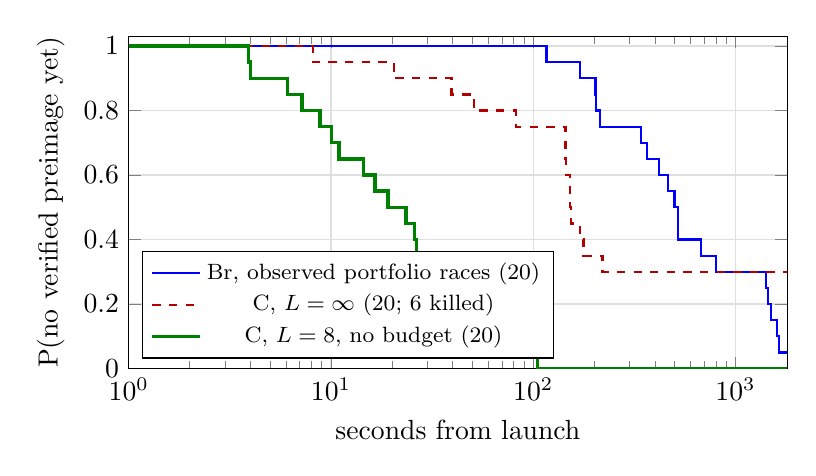
\begin{tikzpicture}
\begin{semilogxaxis}[width=0.82\textwidth,height=5.8cm,xmin=1,xmax=1800,ymin=0,ymax=1.03,
 xlabel={seconds from launch},ylabel={P(no verified preimage yet)},grid=major,grid style={gray!25},
 legend style={font=\footnotesize,at={(0.02,0.03)},anchor=south west}]
\addplot[blue,thick,const plot] coordinates {(1.00,1.0000) (116.33,1.0000) (116.33,0.9500) (170.71,0.9500) (170.71,0.9000) (203.23,0.9000) (203.23,0.8500) (204.88,0.8500) (204.88,0.8000) (213.99,0.8000) (213.99,0.7500) (342.62,0.7500) (342.62,0.7000) (365.44,0.7000) (365.44,0.6500) (418.76,0.6500) (418.76,0.6000) (462.31,0.6000) (462.31,0.5500) (499.60,0.5500) (499.60,0.5000) (520.65,0.5000) (520.65,0.4500) (521.19,0.4500) (521.19,0.4000) (677.01,0.4000) (677.01,0.3500) (800.84,0.3500) (800.84,0.3000) (1411.30,0.3000) (1411.30,0.2500) (1446.66,0.2500) (1446.66,0.2000) (1492.75,0.2000) (1492.75,0.1500) (1607.16,0.1500) (1607.16,0.1000) (1647.70,0.1000) (1647.70,0.0500) (1800.00,0.0500)};\addlegendentry{Br, observed portfolio races (20)}
\addplot[red!70!black,thick,dashed,const plot] coordinates {(1.00,1.0000) (8.12,1.0000) (8.12,0.9500) (20.43,0.9500) (20.43,0.9000) (39.48,0.9000) (39.48,0.8500) (50.94,0.8500) (50.94,0.8000) (81.86,0.8000) (81.86,0.7500) (144.33,0.7500) (144.33,0.7000) (144.40,0.7000) (144.40,0.6500) (144.90,0.6500) (144.90,0.6000) (151.73,0.6000) (151.73,0.5500) (152.18,0.5500) (152.18,0.5000) (153.86,0.5000) (153.86,0.4500) (170.33,0.4500) (170.33,0.4000) (177.40,0.4000) (177.40,0.3500) (220.10,0.3500) (220.10,0.3000) (1800.00,0.3000)};\addlegendentry{C, $L=\infty$ (20; 6 killed)}
\addplot[green!50!black,very thick,const plot] coordinates {(1.00,1.0000) (3.90,1.0000) (3.90,0.9500) (4.01,0.9500) (4.01,0.9000) (6.12,0.9000) (6.12,0.8500) (7.19,0.8500) (7.19,0.8000) (8.83,0.8000) (8.83,0.7500) (10.09,0.7500) (10.09,0.7000) (10.97,0.7000) (10.97,0.6500) (14.52,0.6500) (14.52,0.6000) (16.52,0.6000) (16.52,0.5500) (19.14,0.5500) (19.14,0.5000) (23.51,0.5000) (23.51,0.4500) (25.97,0.4500) (25.97,0.4000) (26.56,0.4000) (26.56,0.3500) (33.12,0.3500) (33.12,0.3000) (39.14,0.3000) (39.14,0.2500) (57.02,0.2500) (57.02,0.2000) (76.72,0.2000) (76.72,0.1500) (100.50,0.1500) (100.50,0.1000) (104.20,0.1000) (104.20,0.0500) (105.37,0.0500) (105.37,0.0000) (1800.00,0.0000)};\addlegendentry{C, $L=8$, no budget (20)}
\end{semilogxaxis}
\end{tikzpicture}
\caption{Phase B, Kaplan--Meier estimates on the development targets. At the cap the estimated
fraction still unsolved is 0\% for $L=8$, 5\% for the portfolio and 30\% for $L=\infty$.}
\end{figure}

\subsection{Why unbounded refinement fails: the lock and memory exhaustion}\label{sec:oom}

\begin{table}[h]\centering\small
\begin{tabular}{@{}lcccc@{}}
\toprule
 & \textbf{terminal jobs} & \textbf{refinements} & \textbf{max descendants} & \textbf{killed}\\
 & \textbf{dispatched / run} & \textbf{retired / run} & \textbf{per parent} & \\
\midrule
$L=\infty$ (20 runs) & 3--100 & 0 & 54--302 & 6\\
$L=8$, no budget (20 runs) & 155--359 & 34--53 & 9--10 & 0\\
\bottomrule
\end{tabular}
\caption{Scheduler behaviour, measured from the event records.}
\end{table}

Under $L=\infty$ the lock recurs: all terminal work is created in the first second, nothing retires,
and the refinement emission rate falls from about 140 per second to 4--29 per second. Six runs were
killed by an external SIGKILL at 272--427\,s. Neither the watcher (which kills only after a verified
solution or a stall) nor the timeout (about 1920\,s) sent it. All six died at 10{,}704--10{,}854
cumulative refinement emissions, while every solved run stayed below that band (the largest reached
10{,}297) (Figure~\ref{fig:oom}). A fixed ceiling reached at a fixed accumulated workload is the
signature of memory exhaustion by the kernel's out-of-memory killer, consistent with never-retired
messages accumulating no-goods and growing persistent solvers. The system log was not inspected, so
this remains an inference (R7 in Table~\ref{tab:open}).

Under $L=8$ the threshold retires 34--53 parents per run and caps descendants at 9--10. The first
wave of terminal jobs is two to five times larger. Terminal dispatch also stops after the first
second, but because about 58 workers stay busy on terminal checks, not because of a lock.

\begin{figure}[h]\centering
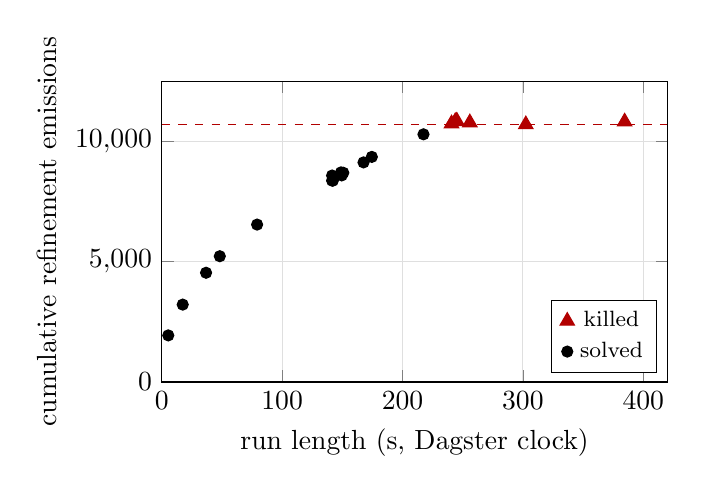
\begin{tikzpicture}
\begin{axis}[width=0.66\textwidth,height=5.4cm,xmin=0,xmax=420,ymin=0,ymax=12500,
 xlabel={run length (s, Dagster clock)},ylabel={cumulative refinement emissions},grid=major,grid style={gray!25},
 legend style={font=\footnotesize,at={(0.98,0.03)},anchor=south east},scaled y ticks=false,
 yticklabel style={/pgf/number format/fixed}]
\addplot[red!70!black,only marks,mark=triangle*,mark size=3pt] coordinates {(255.9,10785) (243.8,10834) (302.4,10704) (245.1,10854) (240.7,10741) (384.5,10820)};\addlegendentry{killed}
\addplot[black,only marks,mark=*,mark size=2pt] coordinates {(141.5,8583) (150.8,8698) (5.4,1937) (142.1,8370) (79.2,6544) (167.6,9129) (174.5,9358) (48.2,5229) (217.4,10297) (141.5,8373) (36.8,4541) (17.4,3217) (148.9,8714) (149.5,8588)};\addlegendentry{solved}
\addplot[red!70!black,dashed,domain=0:420,samples=2,forget plot]{10700};
\end{axis}
\end{tikzpicture}
\caption{$L=\infty$: every killed run died at about 10{,}700--10{,}850 cumulative refinement
emissions (dashed), regardless of how long it had run.}
\label{fig:oom}
\end{figure}

\subsection{Calibration, and why the budgets were dropped}

B1 profiled 2{,}214 completed terminal jobs. The median per-run conflict quantiles were
$B_{50}=39$, $B_{80}=216$, $B_{95}=414$ and $B_{99}=604$. These describe only jobs that
\emph{returned}: without a budget a long check reports nothing until it finishes, so the roughly 58
checks still in flight at each run's end were invisible. Using these quantiles as budgets, as
originally planned, would have cut almost every job into tiny quanta. B3 therefore swept
$\{2{,}000,\ 20{,}000,\ 200{,}000\}$ against a no-budget control at $L=8$.

The budgets fired as intended: 610{,}779, 27{,}271 and 3{,}956 terminal budget-exhaustion events in
total. Every budget nevertheless reduced the yield (1.61 without a budget; 1.21, 0.76 and 0.29 with
one), and the smallest also increased the median and caused the only failed $L=8$ run. Once
refinement retires, terminals are not the bottleneck, and pre-empting them adds polling and re-entry
overhead with no benefit.

\paragraph{Selected configuration, frozen for Phase C:} $L=8$, all budgets zero.

%=============================================================================================
\section{Phase C: Locked Confirmatory Evaluation}\label{sec:phaseC}
%=============================================================================================

\begin{center}\fbox{\parbox{0.94\textwidth}{\small\textbf{Frozen before Phase C.} Nothing below was
changed after the Phase B results were seen.
\begin{itemize}[leftmargin=1.2em,itemsep=1pt]
\item \textbf{Components, in node order:} low16 (nodes 0--1), staged (2--4), part16$_{00}$ (5--6),
part16$_{10}$ (7--8), part16$_{01}$ (9--10), part16$_{11}$ (11--12); 13 nodes. Edges carry
$z_{16}$ (272 bits), or $z_8$ (136 bits) into the staged refinement node, ordered by word
$a_5,\dots,a_{21}$ and then by bit $0..k-1$.
\item \textbf{Dagster:} patch v3, $L=8$, all four conflict budgets 0; flags \flag{-m 4 -q 2 -b 0 -e 0
-i 1 -v 10}; 65 ranks with \flag{-bind-to core}; every run required the exact v3 start-up line.
\item \textbf{Portfolio (Br):} MiniSat~2.2 from Dagster's tree, \flag{-rnd-init -rnd-seed=s}; 64
trajectories pinned to logical CPUs 0--63; seed block $\{64j+1,\dots,64j+64\}$ for repeat $j$; launch
order alternating with C by repeat.
\item \textbf{Run control:} cap 1800\,s; job timeout cap+120\,s then kill; watcher timeout cap+150\,s;
stall rule 60\,s with no new terminal dispatch \emph{and} no terminal job in flight, killing C only.
\item \textbf{Targets:} g10001--g10003 generated as in Appendix~\ref{app:repro}; planted-path and
structural validation required before any run.
\item \textbf{Analysis:} primary metric time to first verified preimage; censoring at each run's end
time; Kaplan--Meier curves; two-sided sign test on decisive pairs; yields on physical core-hours.
\end{itemize}}}\end{center}

With $L=8$ and no budget frozen, each arm ran 10 repeats on each of g10001, g10002 and g10003. None
of these targets played any part in tuning.

\begin{table}[h]\centering\small
\begin{tabular}{@{}llrrrrr@{}}
\toprule
\textbf{target} & \textbf{arm} & \textbf{solved} & \textbf{min (s)} & \textbf{median (s)} & \textbf{max (s)} & \textbf{paired vs Br}\\
\midrule
\multirow{3}{*}{g10001} & C & 10/10 & 7.7 & 25.7 & 153.8 & 10--0 ($p=0.002$)\\
 & C$'$ & 10/10 & 4.2 & 24.7 & 104.3 & 10--0 ($p=0.002$)\\
 & Br & 9/10 & 87.7 & 603.9 & 1298.0 & ---\\
\addlinespace
\multirow{3}{*}{g10002} & C & 10/10 & 11.3 & 28.1 & 110.9 & 10--0 ($p=0.002$)\\
 & C$'$ & 10/10 & 3.7 & 15.5 & 69.9 & 10--0 ($p=0.002$)\\
 & Br & 10/10 & 434.6 & 516.5 & 930.2 & ---\\
\addlinespace
\multirow{3}{*}{g10003} & C & 10/10 & 5.1 & 15.7 & 99.7 & 10--0 ($p=0.002$)\\
 & C$'$ & 10/10 & 45.0 & 159.2 & 597.2 & 8--2 ($p=0.109$)\\
 & Br & 9/10 & 62.4 & 762.0 & 1753.5 & ---\\
\midrule
\multirow{3}{*}{pooled} & C & 30/30 & 5.1 & 26.9 & 153.8 & 30--0 ($p=1.9{\times}10^{-9}$)\\
 & C$'$ & 30/30 & 3.7 & 40.8 & 597.3 & 28--2 ($p=8.7{\times}10^{-7}$)\\
 & Br & 28/30 & 62.4 & 552.6 & 1753.5 & ---\\
\bottomrule
\end{tabular}
\caption{Phase C on the untouched targets: time from launch to the first verified preimage.}
\label{tab:phaseC}
\end{table}

\begin{figure}[h]\centering
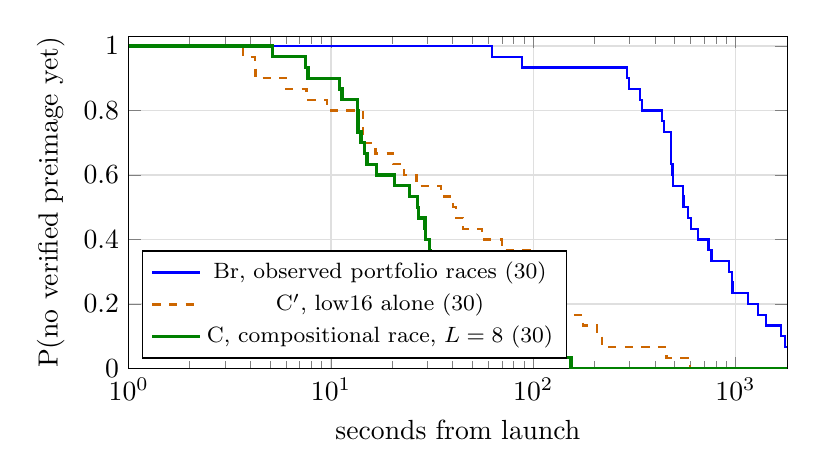
\begin{tikzpicture}
\begin{semilogxaxis}[width=0.82\textwidth,height=5.8cm,xmin=1,xmax=1800,ymin=0,ymax=1.03,
 xlabel={seconds from launch},ylabel={P(no verified preimage yet)},grid=major,grid style={gray!25},
 legend style={font=\footnotesize,at={(0.02,0.03)},anchor=south west}]
\addplot[blue,thick,const plot] coordinates {(1.00,1.0000) (62.37,1.0000) (62.37,0.9667) (87.67,0.9667) (87.67,0.9333) (289.76,0.9333) (289.76,0.9000) (296.69,0.9000) (296.69,0.8667) (335.83,0.8667) (335.83,0.8333) (346.28,0.8333) (346.28,0.8000) (434.62,0.8000) (434.62,0.7667) (444.91,0.7667) (444.91,0.7333) (480.35,0.7333) (480.35,0.7000) (481.44,0.7000) (481.44,0.6667) (481.59,0.6667) (481.59,0.6333) (487.83,0.6333) (487.83,0.6000) (492.78,0.6000) (492.78,0.5667) (551.36,0.5667) (551.36,0.5333) (553.86,0.5333) (553.86,0.5000) (584.98,0.5000) (584.98,0.4667) (603.93,0.4667) (603.93,0.4333) (653.42,0.4333) (653.42,0.4000) (734.72,0.4000) (734.72,0.3667) (761.99,0.3667) (761.99,0.3333) (930.17,0.3333) (930.17,0.3000) (960.30,0.3000) (960.30,0.2667) (966.31,0.2667) (966.31,0.2333) (1150.77,0.2333) (1150.77,0.2000) (1298.01,0.2000) (1298.01,0.1667) (1411.16,0.1667) (1411.16,0.1333) (1676.23,0.1333) (1676.23,0.1000) (1753.45,0.1000) (1753.45,0.0667) (1800.00,0.0667)};\addlegendentry{Br, observed portfolio races (30)}
\addplot[orange!80!black,thick,dashed,const plot] coordinates {(1.00,1.0000) (3.67,1.0000) (3.67,0.9667) (4.21,0.9667) (4.21,0.9333) (4.24,0.9333) (4.24,0.9000) (6.01,0.9000) (6.01,0.8667) (7.57,0.8667) (7.57,0.8333) (9.56,0.8333) (9.56,0.8000) (14.40,0.8000) (14.40,0.7667) (14.45,0.7667) (14.45,0.7333) (14.45,0.7333) (14.45,0.7000) (16.61,0.7000) (16.61,0.6667) (20.24,0.6667) (20.24,0.6333) (22.92,0.6333) (22.92,0.6000) (26.45,0.6000) (26.45,0.5667) (34.96,0.5667) (34.96,0.5333) (40.20,0.5333) (40.20,0.5000) (41.49,0.5000) (41.49,0.4667) (45.04,0.4667) (45.04,0.4333) (55.83,0.4333) (55.83,0.4000) (69.93,0.4000) (69.93,0.3667) (100.50,0.3667) (100.50,0.3333) (104.30,0.3333) (104.30,0.3000) (105.61,0.3000) (105.61,0.2667) (105.88,0.2667) (105.88,0.2333) (114.60,0.2333) (114.60,0.2000) (142.87,0.2000) (142.87,0.1667) (175.57,0.1667) (175.57,0.1333) (207.38,0.1333) (207.38,0.1000) (218.75,0.1000) (218.75,0.0667) (456.26,0.0667) (456.26,0.0333) (597.25,0.0333) (597.25,0.0000) (1800.00,0.0000)};\addlegendentry{C$'$, low16 alone (30)}
\addplot[green!50!black,very thick,const plot] coordinates {(1.00,1.0000) (5.14,1.0000) (5.14,0.9667) (7.50,0.9667) (7.50,0.9333) (7.69,0.9333) (7.69,0.9000) (11.01,0.9000) (11.01,0.8667) (11.32,0.8667) (11.32,0.8333) (13.52,0.8333) (13.52,0.8000) (13.61,0.8000) (13.61,0.7667) (13.62,0.7667) (13.62,0.7333) (14.07,0.7333) (14.07,0.7000) (14.64,0.7000) (14.64,0.6667) (15.07,0.6667) (15.07,0.6333) (16.80,0.6333) (16.80,0.6000) (20.67,0.6000) (20.67,0.5667) (24.42,0.5667) (24.42,0.5333) (26.70,0.5333) (26.70,0.5000) (27.05,0.5000) (27.05,0.4667) (29.12,0.4667) (29.12,0.4333) (29.35,0.4333) (29.35,0.4000) (30.64,0.4000) (30.64,0.3667) (30.98,0.3667) (30.98,0.3333) (34.58,0.3333) (34.58,0.3000) (42.03,0.3000) (42.03,0.2667) (61.52,0.2667) (61.52,0.2333) (67.38,0.2333) (67.38,0.2000) (68.35,0.2000) (68.35,0.1667) (75.28,0.1667) (75.28,0.1333) (99.66,0.1333) (99.66,0.1000) (110.95,0.1000) (110.95,0.0667) (135.61,0.0667) (135.61,0.0333) (153.79,0.0333) (153.79,0.0000) (1800.00,0.0000)};\addlegendentry{C, compositional race, $L=8$ (30)}
\end{semilogxaxis}
\end{tikzpicture}
\caption{Phase C, Kaplan--Meier estimates pooled over the three untouched targets.}
\end{figure}

\begin{figure}[h]\centering
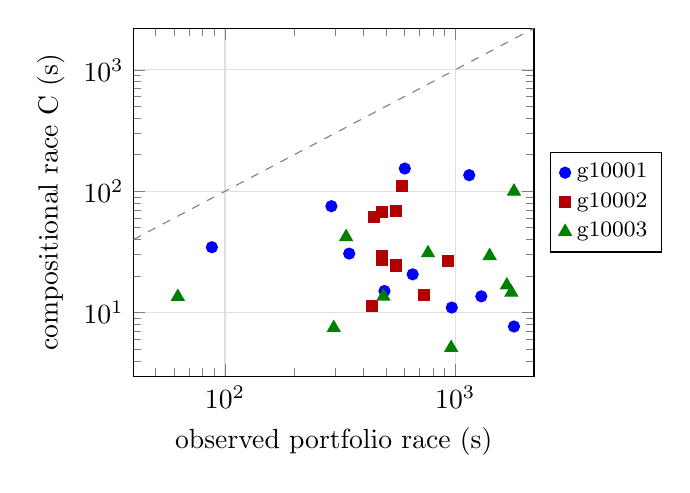
\begin{tikzpicture}
\begin{loglogaxis}[width=0.55\textwidth,height=6cm,xmin=40,xmax=2200,ymin=3,ymax=2200,
 xlabel={observed portfolio race (s)},ylabel={compositional race C (s)},grid=major,grid style={gray!25},
 legend style={font=\footnotesize,at={(1.04,0.5)},anchor=west}]
\addplot[gray,dashed,domain=40:2200,samples=2,forget plot]{x};
\addplot[blue,only marks,mark=*,mark size=2pt] coordinates {(1800.00,7.69) (603.93,153.79) (87.67,34.58) (1150.77,135.61) (492.78,15.07) (966.31,11.01) (1298.01,13.62) (346.28,30.64) (289.76,75.28) (653.42,20.67)};\addlegendentry{g10001}
\addplot[red!70!black,only marks,mark=square*,mark size=2pt] coordinates {(480.35,27.05) (551.36,24.42) (553.86,68.35) (481.59,29.12) (481.44,67.38) (734.72,14.07) (444.91,61.52) (584.98,110.95) (930.17,26.70) (434.62,11.32)};\addlegendentry{g10002}
\addplot[green!50!black,only marks,mark=triangle*,mark size=2.6pt] coordinates {(1411.16,29.35) (1753.45,14.64) (960.30,5.14) (761.99,30.98) (1800.00,99.66) (62.37,13.52) (1676.23,16.80) (296.69,7.50) (487.83,13.61) (335.83,42.03)};\addlegendentry{g10003}
\end{loglogaxis}
\end{tikzpicture}
\caption{Phase C, paired by target and repeat. All 30 points lie below the diagonal: the
compositional race was faster in every pair. Unsolved portfolio races are plotted at 1800\,s.}
\end{figure}

\paragraph{Headline.} The compositional race found a verified 22-round preimage in 30 of 30 runs, with
a median of 26.9\,s, and was faster than the observed portfolio race in every one of the 30 pairs
(10 of 10 on each target, $p=0.002$ per target). The ratio of the pooled median times to first verified preimage is
$552.6/26.9\approx20.6$. This is a ratio of medians, not a parallel speedup over sequential execution,
and not the median of the paired ratios. Its yield of 1.38 verified preimages per physical core-hour
is about 20 times the portfolio's 0.069. There were no kills,
no stalls and no invalid solutions in any arm.

\paragraph{Composition against low16 alone.} C$'$ also solved 30 of 30 and beat the portfolio in 28
of 30 pairs. Against C it won 14 of 30 pairs (C won 16; $p=0.86$). Per target the picture differs:
\begin{itemize}
\item g10001: no difference (4--6);
\item g10002: low16 tends to be faster (2--8, $p=0.11$);
\item g10003: the full race is decisively faster (10--0, $p=0.002$; median 15.7\,s against 159\,s).
\end{itemize}
The trans-round relaxation is the main source of the advantage. The additional components make the
race less sensitive to the target: it stays fast on all three, whereas C$'$ is much slower on
g10003. Since both solved all 30 runs, this is robustness in run time, not in solved fraction. The
full race also more than doubles the yield (1.38 against 0.60 per physical core-hour).

\paragraph{Magnitude, paired.} For each target and repeat let $R_i=T_{\mathrm{Br},i}/T_{\mathrm{C},i}$.
Two portfolio races were censored at 1800\,s; for those, $R_i>1800/T_{\mathrm{C},i}$, and the lower
bound is used. Over the 30 pairs, $R_i$ ranges from 2.5 to 234.1, with median 23.6 and geometric
mean 22.0. Per target the medians are 21.5 (g10001), 17.1 (g10002) and 37.7 (g10003). Because two
entries are lower bounds, these statistics are conservative.

\paragraph{Uncertainty.} The exact (Clopper--Pearson) 95\% interval for the probability that C beats
the portfolio in a pair is $[0.884,\ 1]$ from 30 of 30, and $[0.692,\ 1]$ from 10 of 10 on each
target alone. For C against C$'$ (16 of 30) it is $[0.343,\ 0.717]$, consistent with no
difference. Per-target medians are given in Table~\ref{tab:phaseC}. The pooled median is
descriptive only, since pooling three targets can hide target effects.

\paragraph{Census and yield arms.} The MiniSat census agrees with the races: only 2 of 64 trajectories
per target solved within 1800\,s (g10001: 1331 and 1621\,s; g10002: 126 and 758\,s; g10003: 179 and
1151\,s). The fixed-length \flag{-e 2} runs produced few distinct verified terminal emissions (1, 6
and 5), almost all from the staged component. This count is scheduler-dependent and is reported for
completeness only.

\paragraph{Independent verification.} All 88 successful outcomes (30 C, 30 C$'$ and 28 portfolio
winners) passed the forward verifier at run time: the watcher verifies a model before ending a C or C$'$
run, and the race runner verifies a winner before declaring it. The portfolio's per-seed model files
were not retained after that check, so only the C and C$'$ models could be audited again. In that
stronger audit, all 60 preimages from C and C$'$ were re-verified against
targets regenerated from scratch. The regenerated formulas match the evaluated ones in their header
and in every clause; they differ only in a comment echoing the generator's command line. All 60 are
valid: 57 distinct preimages across the three targets.

%=============================================================================================
\section{Discussion}
%=============================================================================================

\paragraph{What changed between the pilot and the evaluation.} Two things. First, bounded refinement
removed the lock, so the staged pipeline's output is now checked instead of discarded. Second, the
in-flight-aware stall rule stopped the harness from ending runs whose terminal checks were still
live. Together they turn a one-in-five success at 15\,s into 30 of 30 successes with a median of
27\,s on fresh targets.

\paragraph{Why the advantage is large at 22 rounds and absent at 21.} At 21 rounds a single MiniSat
trajectory solves with a median of 154\,s, and 64 of them nearly always include a fast one, so every
method approaches the start-up floor. At 22 rounds only about 3\% of trajectories solve within
1800\,s, so the portfolio relies on rare lucky trajectories. The trace pipelines instead turn the
search into many short, mostly quickly refuted, exact checks of strongly filtered candidates.

\paragraph{CryptoMiniSat.} On one core, CryptoMiniSat was the fastest single solver on the
21-round instance, about ten times faster than MiniSat~2.2, the solver inside Dagster's workers. Its
native-XOR encoding was \emph{slower} than the plain CNF, so the advantage did not come from Gaussian
elimination on the formula's XOR structure, which comprises the adder sums, the schedule and the
Parity rounds (Section~\ref{sec:cms}). At 22 rounds one CryptoMiniSat trajectory found a preimage in 397\,s on a
single core. For scale, the 26.9\,s Dagster median
represents about 1{,}720 worker-core-seconds before counting the master, while that CryptoMiniSat
trajectory used about 397 core-seconds. The two are not directly comparable: they come from different
machines, and the CryptoMiniSat value is a single heavy-tailed observation. Dagster has the better
observed latency; the isolated CryptoMiniSat run used fewer nominal core-seconds; neither observation
establishes a resource-matched ranking. This matters for interpretation. The evaluation compares decomposition against portfolio with the \emph{same} solver,
so a stronger engine would be expected to speed up both arms. The priority next experiment is a repeated,
resource-matched 64-core CryptoMiniSat portfolio (R5). Running CryptoMiniSat as Dagster's worker
engine is outside the scope of this project and is listed as future work only (R13). One seed on one instance is a single trajectory of a heavy-tailed process, not a
ranking of solvers.

\paragraph{Why budgets hurt.} Once refinement retires, the binding constraint is the number of
good candidates generated, not head-of-line blocking at the terminals. Quanta add a poll and a
re-entry per budget, and small quanta fragment the extensions that succeed.

%=============================================================================================
\section{Limitations and future work}\label{sec:future}
%=============================================================================================

The claim established is narrow. At 22 rounds, on three untouched targets with 64 cores, a sound
trace-relaxation decomposition run as a Dagster DAG with bounded refinement finds verified preimages
faster than observed portfolio races of the same MiniSat implementation in every one of 30 paired
runs, with a pooled-median ratio of about 20.6 and a median paired ratio of about 23.6. Table~\ref{tab:open} codes what remains to be established.

\begin{table}[h]\centering\small
\begin{tabularx}{\textwidth}{@{}lLLL@{}}
\toprule
\textbf{Code} & \textbf{Open question} & \textbf{Current evidence} & \textbf{What would establish it}\\
\midrule
R1 & Generality across targets & 3 evaluation targets (and 2 development targets) & At least 10 fresh targets, frozen configuration\\
R2 & Behaviour at 23 rounds and beyond & None & A frozen-configuration probe at $r=23$ with a matched portfolio\\
R3 & Scaling with cores & 64 cores only & 16, 32, 64, 128 workers and sharded instances; verified-solution hazard and unique traces checked, not replicas\\
R4 & Value of composition over low16 & 16--14 overall; decisive on one target only & Many targets, analysed per target; leave-one-component-out runs\\
R5 & \textbf{Priority.} Comparison with stronger-solver portfolios & One core, one seed: CryptoMiniSat about $10\times$ MiniSat at $r=21$, and solved $r=22$ in 397\,s (Table~\ref{tab:cms}) & Repeated, resource-matched 64-core CryptoMiniSat, Kissat and CaDiCaL portfolios on the campaign workstation, many seeds\\
R6 & The best retirement threshold & Only $L\in\{8,\infty\}$ measured & $L\in\{1,2,4,16,64\}$ on development targets\\
R7 & Memory exhaustion as the cause of the $L=\infty$ kills & Fixed-load pattern only & Kernel log, and memory traces per rank\\
R8 & A strict global bound per parent & Worker-local threshold; overshoot up to 2 at $L=8$ & A master-side count of accepted descendants per parent\\
R9 & Execution-model and placement confounds & Same MiniSat, different execution models; 65 ranks on 64 cores, placement not recorded (Table~\ref{tab:res}) & Ablations: Dagster-hosted portfolio; persistent-solver portfolio\\
R10 & Start-up overhead & About 3\,s fixed per Dagster run & Measurements with Dagster pre-warmed or start-up excluded\\
R11 & Behaviour in Dagster's TiniSAT modes & MiniSat mode~4 only & The same controls tested in mode~0\\
R12 & The asymptotic picture & No claim made & Per-round growth for $r=21$--$24$ under the frozen method, compared with the portfolio\\
R13 & Stronger solver inside Dagster & Not attempted; \textbf{outside this project's scope} & CryptoMiniSat (or another engine) as Dagster's worker solver, compared with its own portfolio\\
R14 & Complete provenance & MPICH and compiler versions, Dagster commit and patched-binary hash not recorded (Appendix~\ref{app:prov}) & Recording them in the harness for every run\\
\bottomrule
\end{tabularx}
\caption{Coded list of what remains to be established.}
\label{tab:open}
\end{table}

Beyond these open questions, the patch itself is worth contributing to Dagster in a stricter form
(R8). A master-side count of accepted descendants per parent would give a true global bound, and
retirement could be exposed as a per-node attribute in the DAG file rather than an environment
variable.

%=============================================================================================
\section{Conclusion}
%=============================================================================================

Expressing a sound trans-round relaxation of SHA-1 as a Dagster DAG, and removing one scheduler
pathology with a small, opt-in retirement rule, turns 22-round SHA-1 preimage search from a rare-event
lottery for a 64-core MiniSat portfolio into a computation of about half a minute. On three targets
withheld from all tuning, the compositional race beat the portfolio in 30 of 30 paired runs, and every
preimage was independently verified. Whether the advantage survives a portfolio of a stronger solver,
which a single CryptoMiniSat trajectory suggests is a real possibility, is the next question to
settle. Every claim above is scoped to what was measured.
\appendix

%=============================================================================================
\section{Constructing the instances}\label{app:repro}
%=============================================================================================
Every instance is generated, repaired, decomposed, validated and verified by the following steps,
run from the repository's root. The generator always uses the standard SHA-1 IV, imposes no padding
constraints (all 512 block bits are free), and draws the planted block deterministically from the
seed, so the same generator binary and seed always produce the same instance.
{\footnotesize\begin{verbatim}
# 1. generate: 22 rounds, 160 fixed digest bits, seed 10001, plain CNF
#    (add --xor for the native-XOR variant, used only in the single-solver benchmark)
SHA1GEN_PLANTED_OUT=g10001.cnf.planted \
  bin/sha1gen --attack=preimage --rounds=22 --hash-bits=160 --seed=10001 \
              --cnf --tseitin-adders > g10001.cnf
# 2. repair the DIMACS header (stated 57,543 clauses; true count 57,255)
python3 -c "import sys; sys.path.insert(0,'tools'); from sha1_cnf import Sha1Cnf; \
            Sha1Cnf('g10001.cnf').write_repaired('g10001.repaired.cnf')"
# 3. build the arm-C DAG; this also runs the structural and planted-path validation
python3 tools/compositional_race.py build g10001.cnf --out-prefix C_g10001 \
        --components low16,staged,part16
#    arm C' (low16 alone) uses --components low16
# 4. verify any model independently, by recomputing 22-round SHA-1
python3 tools/verify_preimage.py g10001.cnf MODEL
\end{verbatim}}
The phases are then run by \texttt{scripts/phaseA\_regression.sh} and
\texttt{scripts/runsheet\_demo.sh}, with the settings in the frozen-configuration box of
Section~\ref{sec:phaseC}.

%=============================================================================================
\section{Software provenance}\label{app:prov}
%=============================================================================================
\begin{center}\footnotesize
\begin{tabularx}{\textwidth}{@{}lL@{}}
\toprule
\textbf{Component} & \textbf{Identification}\\
\midrule
Software & this repository, release 1.0. The campaign ran the internal bundle v18 of the same
software (archive SHA-256 \texttt{c0081c5b\dots edce1c1f}, not distributed); the release moves the
generator to \texttt{third\_party/sha1-sat} unchanged and adds the self-test, analysis and provenance
tools\\
Generator (\texttt{sha1-sat} \cite{nossum}, project-patched) & source \texttt{third\_party/sha1-sat/main\_noboost.cc} \texttt{3bcc3634}\dots;
binary on the workstation \texttt{037382ba}\dots; built with \texttt{g++ -O2 -w -std=c++11}\\
Dagster (stock) & upstream commit \textbf{not recorded}; stock \texttt{Worker.cpp} \texttt{ba541d74\dots},
\texttt{minisat\_solver.cc} \texttt{e6461ff8\dots}\\
Dagster patch v3 & diff \texttt{173dbcec\dots}; patch script \texttt{68549a28\dots} (matches the campaign
manifest); patched-binary hash \textbf{not recorded}\\
Dagster build & \texttt{make}: \texttt{mpic++ -ggdb -O3 -std=c++17}, linking glog, CUDD, zlib and
\texttt{stdc++fs}; compiler and library versions \textbf{not recorded}\\
MiniSat 2.2 & the copy in Dagster's source tree, inside Dagster and as the portfolio engine
(engine binary on the workstation \texttt{ab6a3330\dots})\\
MPI & MPICH with the Hydra process manager; version \textbf{not recorded}\\
Processor & AMD Ryzen Threadripper 3990X (64 cores, 128 threads, one socket and NUMA node), recorded after the campaign\\
Operating system & Linux 5.4.0-148-generic; Python 3.8\\
Tools & \texttt{sha1\_cnf.py} \texttt{2f6d2536}\dots, \texttt{verify\_preimage.py} \texttt{4ceeaf28}\dots,
\texttt{compositional\_race.py} \texttt{cd827761}\dots, \texttt{trace\_relaxation.py} \texttt{957a5ce8}\dots, \texttt{watcher.py}
\texttt{10738a59}\dots, \texttt{portfolio\_race.py} \texttt{d08bb6df}\dots, \texttt{runsheet\_demo.sh} \texttt{34c1c365}\dots\\
Single-solver benchmark (Table~\ref{tab:cms}) & separate machine, one core: python-sat 1.9.dev15 (MiniSat 2.2,
CaDiCaL 1.9.5) and pycryptosat 5.17.0 (CryptoMiniSat 5); for XOR files the verifier was extended to
skip XOR lines, a change not present in the campaign bundle\\
Kissat (workstation probe, Section~\ref{sec:cms}) & version \textbf{not recorded}\\
\bottomrule
\end{tabularx}
\end{center}
The items marked \emph{not recorded} are open item R14.

%=============================================================================================
\section{Evidence in the repository}\label{app:evidence}
%=============================================================================================
Every number in the results is regenerated by \texttt{evidence/scripts/derive.py} from the run records
in \texttt{evidence/runs/}, and \texttt{make selftest} checks that they agree.

\begin{center}\footnotesize
\begin{tabularx}{\textwidth}{@{}>{\raggedright\arraybackslash}p{3.2cm}LL@{}}
\toprule
\textbf{In this volume} & \textbf{Evidence} & \textbf{Produced by}\\
\midrule
Phase A & \texttt{evidence/validation/phaseA\_report.txt} & \texttt{scripts/phaseA\_regression.sh}\\
Phases B and C, every run & \texttt{evidence/runs/}, \texttt{evidence/derived/runs.csv} & \texttt{scripts/runsheet\_demo.sh}; \texttt{derive.py}\\
Per-arm times, yields & \texttt{evidence/derived/summary.csv} & \texttt{derive.py}\\
Paired tests, intervals, ratios & recomputed from \texttt{evidence/runs/} & \texttt{tools/report\_stats.py}\\
Lock mechanism ($L=\infty$ against $L=8$) & \texttt{evidence/derived/mechanism.csv} & \texttt{derive.py} from the raw event logs\\
Budget events & \texttt{evidence/derived/budget.csv} & \texttt{derive.py}\\
Census & \texttt{evidence/derived/census.csv}, \texttt{evidence/runs/census/} & \texttt{portfolio/portfolio\_harness.sh}\\
Instances and digests & \texttt{evidence/instances/} & \texttt{bin/sha1gen}; checked by \texttt{make selftest}\\
Checksums; environment & \texttt{evidence/checksums.txt}; \texttt{evidence/provenance.txt} & ---\\
\bottomrule
\end{tabularx}
\end{center}

The run records were stripped of absolute paths and host names before release. The raw campaign
archives and the Dagster event logs contain both, so they are not distributed; they are identified by
SHA-256 in \texttt{evidence/checksums.txt}. The figures for the earlier 21- and 22-round pilot campaigns
in Section~\ref{sec:background} embed their data in this volume's source; those campaigns' raw results
were not retained.

%=============================================================================================
\section{Instance artefacts}\label{app:instances}
%=============================================================================================
SHA-256 of every artefact for the five targets. The DAG file is identical for all five: it holds only
clause-index ranges and edge variables, which depend on the round count and not on the target. The
combined DAG CNF has 57{,}263 clauses: the 57{,}255 exact clauses plus 8 partition unit clauses, two
for each part16 source.
{\scriptsize\setlength{\tabcolsep}{3pt}
\begin{longtable}{@{}lll@{}}
\toprule
\textbf{target} & \textbf{artefact} & \textbf{SHA-256}\\
\midrule\endhead
g10001 & generator output (raw CNF) & \texttt{89e4c3aa62dedb2376b5204cf9f1ccea7220a24fb8aab3f1b98a218f64654716}\\
 & repaired CNF (portfolio input) & \texttt{2088c51da6f0574aba23aa56f0a6cff6b2274508f66ab1ce3c324147943c2367}\\
 & combined DAG CNF (arm C input) & \texttt{178b8cab4042f720004b023285360d3ac8a47e724b4bfee77406affce93f1a2c}\\
 & DAG file & \texttt{a53fb90d4c0f838d1c2931df4d290780ae7620f084bd596bddc258495118e0ac}\\
 & component list & \texttt{8f6889ad7ae0cdec27291cc0bf3d56f0fbddae1c6fcf53563377a500168c6f3b}\\
 & DAG manifest & \texttt{3f37653468f3b4725fe24203a5cddc59715c42c87a680e8d6e4fcb5e3f01b05b}\\
\addlinespace
g10002 & generator output (raw CNF) & \texttt{bfb8b875fd7527c730404a4cbd198db62de797f72466d7a67e837e43d2d12ede}\\
 & repaired CNF (portfolio input) & \texttt{c091f569fcb05764cc9e0f91e5ef142bfc38d64b4db813dcdba569413dd6ba53}\\
 & combined DAG CNF (arm C input) & \texttt{d52ba94be86b9fe44779c53aa7abfa7e12229d4bbcb9f4c03cffbd8273aa5e4d}\\
 & DAG file & \texttt{a53fb90d4c0f838d1c2931df4d290780ae7620f084bd596bddc258495118e0ac}\\
 & component list & \texttt{e85e056c3576dfd423e874f4a1fd888c4d89186c8cf3aa4df8c8b6165b120b1a}\\
 & DAG manifest & \texttt{94775dabd2533160468a61636050d151325911caa060344d94d8658e7cb4eb22}\\
\addlinespace
g10003 & generator output (raw CNF) & \texttt{57d767b70ad448670d0d8a3dc313f3732ee6f8529beb56ccbf769a5c29beb690}\\
 & repaired CNF (portfolio input) & \texttt{4cf2a515b3b9619b668399fd34ea9040f13691ecc73e61d34d459748403f9494}\\
 & combined DAG CNF (arm C input) & \texttt{52202502dc8d55f7c956b73b70329c8b4997b146c267934b1bed9e822c607d27}\\
 & DAG file & \texttt{a53fb90d4c0f838d1c2931df4d290780ae7620f084bd596bddc258495118e0ac}\\
 & component list & \texttt{6b17aa8ed04d259289c6011f1802c51dd3035680680ab20b9bb82b2f5d980d83}\\
 & DAG manifest & \texttt{191b64debe276c1efc8d0a9c936636c59afad807e57d2316f3a53de3b4348bed}\\
\addlinespace
g10004 & generator output (raw CNF) & \texttt{2974f77e12374fdb87d862c491421c5abee87a05dcc0406254d5cbec7594f19b}\\
 & repaired CNF (portfolio input) & \texttt{d5acc8c75c6174a563252a00326221eab99a2fdd05eb06fdbc8eab2edf659433}\\
 & combined DAG CNF (arm C input) & \texttt{1f654945d41ef9f9e0173a380c6cc7c7788d536ef0e0c1518a299a3038bbd9ad}\\
 & DAG file & \texttt{a53fb90d4c0f838d1c2931df4d290780ae7620f084bd596bddc258495118e0ac}\\
 & component list & \texttt{2fa50e76cd4e8efb335702e3ec82f7f37653d85dae01f8242c864eae3d9fee8e}\\
 & DAG manifest & \texttt{5d09380f011dccc3b4d08378c4a47ff1f0deb2beb73f54ada9f5009b50126aa2}\\
\addlinespace
g10005 & generator output (raw CNF) & \texttt{93366b2eb0784d073dcfb9c96a7cd23560163eedd559efbb951e78213f02b2dd}\\
 & repaired CNF (portfolio input) & \texttt{0321f7247564ba19a7af6aa541084de3bdd6b7f294b0dd69df540bbf8b003c56}\\
 & combined DAG CNF (arm C input) & \texttt{41f0aff7f62b24142c18b74d159e6e4cd10c9b62c2b8204b9e495a0d59b6e215}\\
 & DAG file & \texttt{a53fb90d4c0f838d1c2931df4d290780ae7620f084bd596bddc258495118e0ac}\\
 & component list & \texttt{5f3e2a3b0dfccbb3858bd88e3a907da8be6ffc8372c88330234e0f3496da6218}\\
 & DAG manifest & \texttt{a56103585322aed04e78332d98da9818ce5f30bc9219fb6c631bd7e71f1510f1}\\
\bottomrule
\end{longtable}}

The planted message blocks, as 16 big-endian 32-bit words $W_0\dots W_{15}$ in hexadecimal. They were
used only to validate the DAG constructions and to compute the digests in Table~\ref{tab:inst}; no
solver ever received them.
{\scriptsize\setlength{\tabcolsep}{3pt}
\begin{longtable}{@{}ll@{}}
\toprule
\textbf{target} & \textbf{planted block ($W_0\dots W_7$, then $W_8\dots W_{15}$)}\\
\midrule\endhead
g10001 & \texttt{700aeca76f00370516936c6b37f7eade3cac2a990437ee87327b9ada017e06cb}\\ & \texttt{1db6201315a73799214357c91a11b7284d01d9f448d6ee9151055e7b01d98c23}\\
g10002 & \texttt{3314e61c5e3a8bd649494f686094de972704265e477d1f682e4790a75527dd14}\\ & \texttt{2cd7f328380ef58a1441bd66726a09016631a9593da2fa924d9b60e81662828c}\\
g10003 & \texttt{7500e7e8096497b227a804145bca53d33f6af8ea0d7e8d04192d64136485ea10}\\ & \texttt{37dde27440a420e60189db923dca69bd4a73c1656271ffae7627b5d45ffeb308}\\
g10004 & \texttt{355def84411d705514cc40456e01877919d18dcf1e973d4f2ec162cc5c79219f}\\ & \texttt{18b491217b017b58671a3d52408cfbb418ad5e5a2c637ec8119aa31c6ef2dde6}\\
g10005 & \texttt{30045e243cde4a755f61dfe504a03e99656c466f44d7996f786d5c6c1c782abf}\\ & \texttt{23fe33c11cf7797864a830f2165f76d47f6a8afa44873ee854f030bc471deb06}\\
\bottomrule
\end{longtable}}

\section{Patch listing}\label{app:patch}

The diff quotes Dagster source code, which remains under Dagster's licence (GPL-2.0-or-later);
this appendix gives the complete diff (SHA-256 \texttt{173dbcec\dots c6636892}), unchanged except that lines longer than 92 characters are
wrapped (marked by a trailing \texttt{\textbackslash}).

\paragraph{\texttt{Worker.cpp}: declarations for state defined in the MiniSat wrapper.}
{\scriptsize\begin{verbatim}
@@ -1,3 +1,12 @@
+// DAGSTER_BOUNDED_PATCH v3
+#include <cerrno>
+#include <cstdlib>
+#include <string>
+#include <functional>
+#include <algorithm>
+extern long long dagster_minisat_budget; extern const char* dagster_minisat_role;
+extern long long dagster_minisat_conflicts_this_call; extern long long dagster_minisat_conf \
  +    licts_total;
+extern bool dagster_minisat_budget_exhausted;
 /*************************
 Copyright 2020 Mark Burgess
\end{verbatim}}

\paragraph{\texttt{Worker.cpp}: parsing and validating the controls; per-message state.}
{\scriptsize\begin{verbatim}
@@ -61,6 +70,26 @@
 //
 void Worker::loop() {
   int solution_count = 0;
+  // ---- DAGSTER_BOUNDED_PATCH v3: parse and validate controls (fatal on invalid input) -- \
  +    --
+  auto env_int = [](const char* name) -> long long {
+    const char* v = getenv(name);
+    if (v == NULL || *v == '\0') return -1;                    // unset
+    char* end = NULL; errno = 0;
+    long long x = strtoll(v, &end, 10);
+    if (errno != 0 || end == v || *end != '\0' || x < 0 || x > 1000000000000LL)
+      LOG(FATAL) << "DAGSTER_PATCH: invalid value " << name << "=" << v << " (need integer  \
  +    0..1e12)";
+    return x;
+  };
+  const long long max_intermediate = std::max(0LL, env_int("DAGSTER_MAX_INTERMEDIATE_SOLUTI \
  +    ONS"));
+  const long long q_default = std::max(0LL, env_int("DAGSTER_MINISAT_CONFLICT_QUANTUM"));
+  auto role_budget = [&](const char* name) { long long v = env_int(name); return v < 0 ? q_ \
  +    default : v; };
+  const long long budget_terminal = role_budget("DAGSTER_MINISAT_TERMINAL_CONFLICT_BUDGET") \
  +    ;
+  const long long budget_intermediate = role_budget("DAGSTER_MINISAT_INTERMEDIATE_CONFLICT_ \
  +    BUDGET");
+  const long long budget_source = role_budget("DAGSTER_MINISAT_SOURCE_CONFLICT_BUDGET");
+  LOG(INFO) << "WORKER " << comms->world_rank << ": DAGSTER_PATCH v3 L=" << max_intermediat \
  +    e
+            << " budget_terminal=" << budget_terminal << " budget_intermediate=" << budget_ \
  +    intermediate
+            << " budget_source=" << budget_source;
+  long long msg_solutions = 0; std::string msg_key; size_t msg_digest = 0;
   Message* m2 = new Message();
   Message* working_message = NULL;
   while (true) {
\end{verbatim}}

\paragraph{\texttt{Worker.cpp}: the per-message key, and the role-dependent budget before each call.}
{\scriptsize\begin{verbatim}
@@ -82,13 +111,31 @@
       VLOG(4) << "I HAVE RECIEVED MESSAGE: " << *m;
       message_index++;
       initialise_solver_from_message(m);
+      { std::string key = std::to_string(m->to) + ":";
+        for (size_t q = 0; q < m->assignments.size(); q++) key += std::to_string(m->assignm \
  +    ents[q]) + ",";
+        if (key != msg_key) { msg_key = key; msg_solutions = 0; msg_digest = std::hash<std: \
  +    :string>{}(key); } }
     }
     
     if ((message_tag == MPI_TAG_POLL_FOR_REASSIGNMENT) || (message_tag == MPI_TAG_NEW_ASSIG \
       NMENT)) { // proceed to solving for a loaded message
       VLOG(4) << "WORKER " << comms->world_rank << ": generating new solution";
       solution_count = 0;
 generate_new_result:
+      // role of the node being solved: root (self-loop reverse edge), terminal, or interme \
  +    diate
+      { int nd = m2->to;
+        bool is_root = dag->reverse_connections[nd].size() == 1 && dag->reverse_connections \
  +    [nd][0] == nd;
+        bool is_terminal = dag->forward_connections[nd].empty();
+        dagster_minisat_role = is_root ? "source" : (is_terminal ? "terminal" : "intermedia \
  +    te");
+        dagster_minisat_budget = is_root ? budget_source : (is_terminal ? budget_terminal : \
  +     budget_intermediate); }
       int result = solve_and_generate_message(m2, working_message);
+      if (minisat_mode) VLOG(3) << "WORKER " << comms->world_rank << ": MINISAT_RESULT node \
  +    =" << m2->to << " role=" << dagster_minisat_role
+              << " msg=" << std::hex << msg_digest << std::dec << " result=" << result
+              << " conflicts_this_call=" << dagster_minisat_conflicts_this_call
+              << " conflicts_total=" << dagster_minisat_conflicts_total;
+      if (minisat_mode && result == 2 && dagster_minisat_budget_exhausted)
+        LOG(INFO) << "WORKER " << comms->world_rank << ": MINISAT_BUDGET_EXHAUSTED node=" < \
  +    < m2->to
+                  << " role=" << dagster_minisat_role << " msg=" << std::hex << msg_digest  \
  +    << std::dec
+                  << " conflicts_this_call=" << dagster_minisat_conflicts_this_call
+                  << " conflicts_total=" << dagster_minisat_conflicts_total;
       //VLOG(2) << "WORKER " << comms->world_rank << ": generated made " << solver->decisio \
       ns << " decisions, including "<<solver->num_set_literal << " sets, and " << solver->n \
       Conflicts << " conflicts, generating result " << result << " for message " << m2->to;
       VLOG(4) << "WORKER " << comms->world_rank << ": generated solution " << result;
       if (result == 0) {
\end{verbatim}}

\paragraph{\texttt{Worker.cpp}: counting descendants and retiring the parent.}
{\scriptsize\begin{verbatim}
@@ -101,8 +148,14 @@
         VLOG(4) << "WORKER " << comms->world_rank << ": Solution message mapped to: " << *m \
       2;
         comms->send_message(0, MPI_TAG_SOLUTION, m2); // send the full solution to master
         solution_count++;
+        msg_solutions++;
         VLOG(4) << "WORKER " << comms->world_rank << ": resetting sathandler";
-        if ((!reset_solver_for_next_solution(m2)) || (command_line_arguments.ENUMERATE_SOLU \
  -    TIONS==3)) { // request for assignment if finished, or if enumerate_solutions mode 3  \
       - assuming only one solution to each dag node message
+        bool is_root2 = dag->reverse_connections[m2->to].size() == 1 && dag->reverse_connec \
  +    tions[m2->to][0] == m2->to;
+        bool intermediate = !is_root2 && !dag->forward_connections[m2->to].empty();
+        bool retire = intermediate && max_intermediate > 0 && msg_solutions >= max_intermed \
  +    iate;
+        if (retire) LOG(INFO) << "WORKER " << comms->world_rank << ": REFINEMENT_RETIRE nod \
  +    e=" << m2->to
+                              << " msg=" << std::hex << msg_digest << std::dec << " emitted \
  +    _by_this_worker=" << msg_solutions;
+        if (retire || (!reset_solver_for_next_solution(m2)) || (command_line_arguments.ENUM \
  +    ERATE_SOLUTIONS==3)) { // request for assignment if finished, or if enumerate_solutio \
       ns mode 3 - assuming only one solution to each dag node message
           VLOG(3) << "WORKER " << comms->world_rank << ": finished generating new solutions \
       , sending assignment request";
           comms->send_tag(0, MPI_TAG_REQUEST_FOR_ASSIGNMENT);
         } else if (solution_count >= command_line_arguments.sat_solution_interrupt) {
\end{verbatim}}

\paragraph{\texttt{minisat\_solver.cc}: per-call budget and statistics.}
{\scriptsize\begin{verbatim}
@@ -1,3 +1,4 @@
+// DAGSTER_BOUNDED_PATCH v3
 /*************************
 Copyright 2021 Mark Burgess
@@ -33,6 +34,12 @@
 #include "SimpSolver.h"
 
 using namespace Minisat;
+// ---- DAGSTER_BOUNDED_PATCH v3: per-call budget set by the Worker, and per-call statistic \
  +    s ----
+long long dagster_minisat_budget = 0;
+const char* dagster_minisat_role = "unset";
+long long dagster_minisat_conflicts_this_call = 0;
+long long dagster_minisat_conflicts_total = 0;
+bool dagster_minisat_budget_exhausted = false;
 
 
 MinisatSolver::MinisatSolver(Cnf* cnf) {
@@ -148,9 +155,21 @@
     if (absent)
       lits.push(this->unit_assignments[i]);
   }
-  bool ret = solve(lits, false, false);
-  DB(printf("returning %i\n",ret);)
-  return ret;
+  long long c_entry = (long long) conflicts;
+  dagster_minisat_budget_exhausted = false;
+  int out;
+  if (dagster_minisat_budget > 0) {            // fresh quantum, relative to the current co \
  +    unt
+    setConfBudget(dagster_minisat_budget);
+    lbool r = solveLimited(lits, false, false);
+    budgetOff();
+    if (r == l_True) out = 1; else if (r == l_False) out = 0;
+    else { out = 2; dagster_minisat_budget_exhausted = true; }
+  } else {
+    out = solve(lits, false, false) ? 1 : 0;
+  }
+  dagster_minisat_conflicts_this_call = (long long) conflicts - c_entry;
+  dagster_minisat_conflicts_total = (long long) conflicts;
+  return out;
 }
\end{verbatim}}



%=============================================================================================
\section{Phase C per-run records}
%=============================================================================================
{\small\begin{longtable}{@{}rrrlrlrl@{}}\toprule target & rep & C (s) & C winner & C$'$ (s) & & Br (s) & Br winner\\\midrule\endhead
g10001 & 1 & 7.7 & staged & 104.3 & & unsolved & seed --\\
g10001 & 2 & 153.8 & staged & 6.0 & & 603.9 & seed 185\\
g10001 & 3 & 34.6 & staged & 4.2 & & 87.7 & seed 250\\
g10001 & 4 & 135.6 & staged & 22.9 & & 1150.8 & seed 301\\
g10001 & 5 & 15.1 & staged & 7.6 & & 492.8 & seed 381\\
g10001 & 6 & 11.0 & staged & 35.0 & & 966.3 & seed 407\\
g10001 & 7 & 13.6 & staged & 100.5 & & 1298.0 & seed 469\\
g10001 & 8 & 30.6 & staged & 40.2 & & 346.3 & seed 515\\
g10001 & 9 & 75.3 & staged & 26.4 & & 289.8 & seed 584\\
g10001 & 10 & 20.7 & staged & 4.2 & & 653.4 & seed 666\\
g10002 & 1 & 27.0 & staged & 9.6 & & 480.4 & seed 128\\
g10002 & 2 & 24.4 & staged & 16.6 & & 551.4 & seed 142\\
g10002 & 3 & 68.3 & staged & 20.2 & & 553.9 & seed 197\\
g10002 & 4 & 29.1 & staged & 14.5 & & 481.6 & seed 310\\
g10002 & 5 & 67.4 & staged & 14.5 & & 481.4 & seed 365\\
g10002 & 6 & 14.1 & staged & 55.8 & & 734.7 & seed 394\\
g10002 & 7 & 61.5 & staged & 41.5 & & 444.9 & seed 462\\
g10002 & 8 & 110.9 & staged & 3.7 & & 585.0 & seed 558\\
g10002 & 9 & 26.7 & staged & 14.4 & & 930.2 & seed 627\\
g10002 & 10 & 11.3 & staged & 69.9 & & 434.6 & seed 656\\
g10003 & 1 & 29.3 & staged & 597.2 & & 1411.2 & seed 72\\
g10003 & 2 & 14.6 & staged & 105.9 & & 1753.5 & seed 187\\
g10003 & 3 & 5.1 & low16 & 105.6 & & 960.3 & seed 249\\
g10003 & 4 & 31.0 & staged & 207.4 & & 762.0 & seed 266\\
g10003 & 5 & 99.7 & staged & 114.6 & & unsolved & seed --\\
g10003 & 6 & 13.5 & low16 & 142.9 & & 62.4 & seed 439\\
g10003 & 7 & 16.8 & low16 & 218.7 & & 1676.2 & seed 495\\
g10003 & 8 & 7.5 & staged & 45.0 & & 296.7 & seed 544\\
g10003 & 9 & 13.6 & low16 & 175.6 & & 487.8 & seed 619\\
g10003 & 10 & 42.0 & low16 & 456.3 & & 335.8 & seed 662\\
\bottomrule\end{longtable}}


\begin{thebibliography}{9}
\bibitem{fips180} National Institute of Standards and Technology. \emph{Secure Hash Standard (SHS)}. FIPS PUB 180-4, 2015.
\bibitem{nossum} V.~Nossum. \emph{SAT-based preimage attacks on SHA-1}. Master's thesis, University of Oslo, 2012. Software: \texttt{sha1-sat}.
\bibitem{tseitin} G.~S.~Tseitin. On the complexity of derivation in propositional calculus. In \emph{Studies in Constructive Mathematics and Mathematical Logic, Part II}, 1968.
\bibitem{minisat} N.~E{\'e}n and N.~S{\"o}rensson. An extensible SAT-solver. In \emph{Theory and Applications of Satisfiability Testing (SAT)}, 2003.
\bibitem{cms} M.~Soos, K.~Nohl and C.~Castelluccia. Extending SAT solvers to cryptographic problems. In \emph{Theory and Applications of Satisfiability Testing (SAT)}, 2009.
\bibitem{burgess2022dagster} M.~A.~Burgess, C.~Gretton, J.~Milthorpe, L.~Croak, T.~Willingham and A.~Tiu. Dagster: parallel structured search with case studies. In \emph{PRICAI 2022: Trends in Artificial Intelligence}, LNCS 13629, pages 75--89. Springer, 2022. \url{https://doi.org/10.1007/978-3-031-20862-1_6}
\bibitem{burgess2023dagster} M.~A.~Burgess, C.~Gretton, J.~Milthorpe, L.~Croak, T.~Willingham and A.~Tiu. Dagster: parallel structured search. In \emph{Proceedings of the Thirty-Seventh AAAI Conference on Artificial Intelligence}, Student Papers and Demonstrations, volume 37, pages 16404--16406. AAAI Press, 2023. \url{https://doi.org/10.1609/aaai.v37i13.27060}
\end{thebibliography}
\end{document}
